\documentclass[twocolumn]{article}
\usepackage[english]{babel}
\usepackage[a4paper,top=2cm,bottom=2cm,left=3cm,right=3cm,marginparwidth=1.75cm]{geometry}
\usepackage{derivative}
\usepackage{amsmath,amssymb}
\usepackage{subcaption}
\usepackage{makecell}
\usepackage{float}
\usepackage[table]{xcolor}
\usepackage{graphicx}
\usepackage{placeins}
\usepackage[colorlinks=true, allcolors=blue]{hyperref}
\usepackage[toc,page]{appendix}
\usepackage{pgfgantt}
\usepackage{booktabs}
\usepackage{rotating}
\usepackage{makecell}
\usepackage{pgfplots}
\pgfplotsset{width=10cm,compat=1.9}
\usepackage{csquotes}
\usepackage{url}


\begin{document}

\begin{titlepage}
    \centering
    \vspace*{\fill}
    
    {\LARGE \textbf{Development of a Deep Learning Denoising and Super-Resolution Framework for Micro-MRI} \par}
    \vspace{0.5cm}

    {\Large Darío Conejo Rupp, Magali De Poortere, Wolf De Mits, Fea Suy, Daan Vleurick \par}
    \vspace{2cm}

    {\large Research group: Infinity Lab and Medical Imaging and Signal Processing (Medisip) \par}
    \vspace{0.2cm}

    {\large Promotors: Stefaan Vandenberghe, Christian Vanhove \par}
    \vspace{0.2cm}

    {\large Supervisors: Florence Muller, Maya Abi Akl, Boris Vervenne, Melissa Lajtos \par}

    \vspace{2cm}

    {\large {Project in het kader van het Vakoverschrijdend Projectvak in de bachelor Biomedische ingenieurstechnieken} \par}
    {\large {VOP 1} \par}
    {\large \textbf{Academic year 2024-2025} \par}

    \vspace*{\fill}
\end{titlepage}

\newpage
\onecolumn
\begin{abstract}
Magnetic resonance imaging (MRI) is a non‐invasive imaging technique that uses magnetic fields and radiofrequency pulses to generate detailed anatomical images. 
Micro-MRI, a preclinical imaging modality, offers excellent soft tissue contrast for anatomical visualization in rodent models. 
However, achieving an optimal balance between spatial resolution, acquisition time, and signal to noise ratio (SNR) remains challenging. 
In this study a deep learning denoising and super-resolution framework for micro-MRI to reduce scan time while enhancing spatial resolution is developed. 
A total of 24 mice were scanned using a $7$T Bruker Pharmascan micro-MRI scanner. For each T2-weighted image, 2 scans were acquired: a 1-minute low-resolution scan and a 12-minute high-resolution scan. 
Following data acquisition, the data was pre-processed. The pre-processing included (1) removing bad slices, (2) cropping the images, (3) put them into Zarr arrays, (4) normalize them and (5) padding and random flipping. 
After the data was pre-processed, a U-Net architecture was optimized by exploring different hyperparameters. 
The optimizer, scheduler, features main, features skip, upsampling method, downsampling method, learning rate, loss function, activation function, batch size and residual learning were trained via Optuna. 
After getting the best hyperparameters the model was trained with and without super-resolution. To evaluate the model performance different strategies were used. 
The following methodologies were chosen: mean squared error (MSE), structural similarity index measure (SSIM), contrast-to-noise ratio (CNR) and visual comparison. 
In addition, a second model, namely anchored path diffusion denoising model, was designed and trained.
\end{abstract}\hspace{15pt}
\newpage

\tableofcontents
\newpage
\onecolumn
\listoffigures
\listoftables

\newpage
\section*{Acknowledgements}
\addcontentsline{toc}{section}{Acknowledgements}
This project was carried out by a group of five individuals, including Darío Conejo Rupp, Magali De Poortere, Wolf De Mits, Fea Suy and Daan Vleurick. 
The collaboration went smoothly and greatly contributed to achieve a successful result. Every Wednesday, the five of us came together to help each other and discuss the next steps towards our goal. 
A detailed schedule and division of labor can be found in Appendix \ref{appendix:Division of tasks}. This schedule was made by the promotors and supervisors. 
It was a feasible schedule so this schedule was followed.  \\

Wolf focused on the anchored path diffusion. Fea and Magali focused on the literature study, report and organization. 
They also give their input to develop the deep learning together with Daan and Darío.

We want to thank Prof. Vandenberghe, Prof. Vanhove, Florence Muller, Boris Vervenne, Maya Abi Akl and Melissa Lajtos. 
Also, we would like to express out gratitude to the MEDISIP team for providing the opportunity to use the INFINITY lab. 
Each of the individuals mentioned offered their support and played an important role in the success of this project. \\

Finally, we would like to thank Niels Verhelst and Joran Courtens for acquiring the mouse scans during the 2024 summer internship and for their preliminary contributions to the research.



\newpage
\section{Introduction}

MRI is a non‐invasive imaging technique that uses magnetic fields and radio frequency pulses to generate detailed anatomical images. 
Micro-MRI is a non-invasive preclinical imaging modality that provides excellent soft tissue contrast for anatomical visualization in rodent models. 
To visualize the animal's anatomy with sufficient details a high spatial resolution is important. Reducing voxel size improves spatial resolution but also decreases the signal and lowers the SNR. 
On the other hand, increasing acquisition time can enhance signal quality and SNR. However, this increases the risk of artefacts, blurring, and motion-related distortions. 
Additionally, longer scan times are often impractical in real-life imaging workflows, where efficiency and throughput are essential. 
A good balance between spatial resolution, acquisition time and SNR is needed.
In recent years, deep learning has emerged as a tool to address this trade-off between scan duration, resolution and image quality. 
While more traditional techniques relied on manual tuning or fixed algorithms, deep learning methods can learn to restore fine details and reduce noise directly from examples of high and low quality images. 
The study of the cross-course project (vakoverschrijdend project) proposes to develop a deep learning model that can predict a high-resolution image (12 minutes acquisition time) from a low resolution image (obtained in just 1 minute of acquisition time). 
This approach aims to reduce the acquisition time while achieving a good resolution and a high SNR \cite{brown2014magnetic}. 

\twocolumn
\section{Materials and Methods}
\subsection{Safety measures}

To avoid contamination of the lab, the operator must wear a hairnet, face mask, lab coat, latex gloves and shoe covers. 
Metallic objects can be pulled into the MRI or disrupt the magnetic field, so they should be left outside the MRI room. 
The Infinity lab at UZ Ghent Hospital Campus where this research was conducted also contains X-ray and PET/SPECT systems. 
While X-ray exposure is monitored with personal dosimeters, the Geiger counter at the lab exit is used to detect possible contamination from radioactive tracers used in PET/SPECT imaging.

\subsection{Preparation and calibration }

All imaging was performed using a Bruker PharmaScan system operating at 7 Tesla designed for small animal imaging \cite{bruker2025pharmascan}. 
A rat brain surface coil from Rapid Biomedical was used for the scans that were already provided (see later) and the scans acquired during this project. 
The coil remained unchanged throughout the experiment to maintain uniformity in data acquisition.
Before the acquisition sequence began, the mouse needed to be placed inside the scanner properly. 
The mouse was positioned with either the head-thorax region or thorax-abdomen region in the field of view (see Figure~\ref{fig:head-thorax}). 
Supports and tape were used to fixate the mouse. 

\begin{figure}[H]
    \centering
    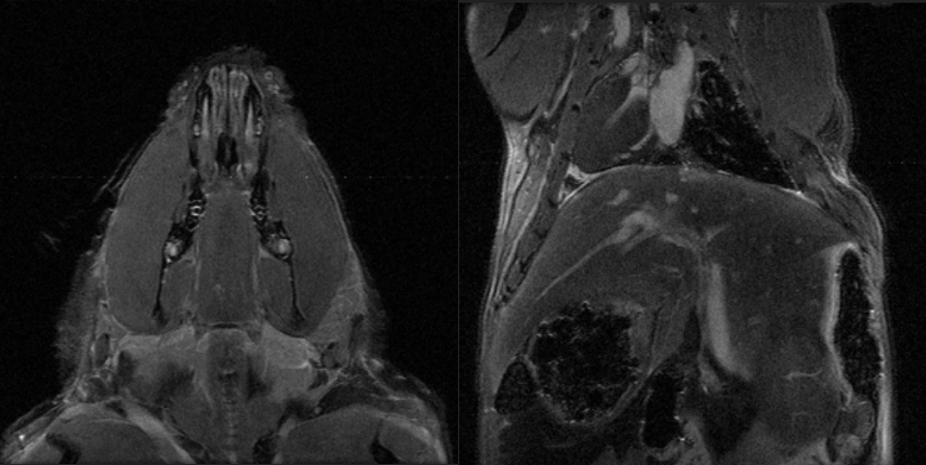
\includegraphics[width=0.95\linewidth]{head-thorax.png}
    \caption{Left figure shows the head-thorax region and the right figure shows the thorax-abdomen region.}
    \label{fig:head-thorax}
\end{figure}

The acquisition sequence consisted of multiple steps to fine-tune the system before image acquisition began: 

\begin{enumerate}
\item svWobble scan: svWobble was only performed at the start of the first scan session. It helps the system determine how much water is present in the coil and fine-tunes the scanner accordingly. 
This step is especially necessary when switching between different animal species, as the water content in the coil may vary. 
If the same type of sample (e.g., the same mouse model) is used throughout the experiment, svWobble does not need to be repeated for following scans.
\item Tripilot scan:  short, preliminary scan that allows the user to define the field-of-view (FOV) that needs to be acquired. 
This step generates 3 orthogonal views: axial, sagittal and coronal. A boundary box is then manually defined to encompass the required FOV, ensuring the right structures are within the FOV. 
Especially important is the phase direction, where the FOV must cover the entire subject.
\end{enumerate}

\subsection{Performing the MRI scan}

Once the mouse was correctly positioned and FOV was defined, the process of acquiring 3D MRI data was started. 
This was done for each mouse for both the head-thorax region and the thorax-abdomen region. 
The following sequence was performed: axial default, axial fast, coronal default, coronal fast, sagittal default and lastly sagittal fast. 
In this case ``default'' stands for a 12-minute scan and ``fast'' for a 1-minute scan.

All scans were acquired using a T2-weighted RARE (rapid acquisition with refocused echoes) sequence. 
This sequence is often chosen in preclinical imaging because it produces images that have high contrast between different soft tissues. 
T2-weighted images work by highlighting differences in transverse relaxation time, which reflects how quickly protons lose phase coherence after excitation by a radio frequency pulse. 
This signal decay changes depending on its interaction within different types of tissues. 
Shorter T2's, found in tissues such as muscle and fat, mean that the signal will decay very fast while tissues with a longer T2, for example fluids, retain the signal longer. 
This will result in fluids appearing brighter than muscle and fat in the image. 

From a technical perspective, the T2-weighted contrast is created by correctly selecting the echo time (TE) and the repetition time (TR). 
The echo time is the time between the initial radio frequency pulse and the measured MRI signal. 
A longer TE allows more time for tissues with a short T2 to lose their signal, resulting in them looking darker on the image. 
Tissues with longer T2 values maintain more signal and will look brighter. Repetition time (TR) refers to the time between successive excitations of the same tissue slice. 
Specifically for T2-weighted images a longer TR is used, minimizing the influence of T1 relaxation. For this study a TE of 37.1ms and TR of 4000ms are used. 
This provides a strongly T2-weighted image \cite{chavhan2009t2star}\cite{mrimaster2024}.  


After each image sequence is completed, they are reviewed to check for any misalignment, artifacts, or other issues to ensure accuracy and quality. 

\subsection{Image Datasets}

Below in Table ~\ref{tab:mri} the parameters can be found used for the 1-minute low resolution and 12-minute high resolution scans. 
These values were selected in function of acquisition time, image quality and SNR. 
The matrix size determines the level of detail in an image with the high-resolution scan (300x300) capturing finer structures compared to that of the low-resolution scan (150x150). 
Other parameters such as repetition time, echo time and thickness remained constant for consistency. The field of view also stays the same at 3 cm x 3 cm to capture the same region of interest. 
An important difference between the two scans is the in-plane resolution. The lower this value the higher resolution the visualisation. 
The 12-minute scan (0,01 cm/pixel) is more precise while the 1-minute scan (0,02 cm/pixel) is faster but has less detail. 
To significantly enhance SNR by reducing noise, the high-resolution scan uses five averages per slice.\\
\\
In the summer of 2024 an internship was done by Verhelst Niels and Courtens Joran \cite{verhelst2025denoising}. 
The data that they acquired was used in combination with the data acquired in this project. During the internship 19 mice were scanned. 
In the project the data of 5 mice were acquired.
 

\begin{table}[h]
\centering
\resizebox{0.97\linewidth}{!}{  % Schaal de tabel tot 80% van de kolombreedte
\begin{tabular}{l|c|c}
\toprule
 & \textbf{1 min (low-res)} & \textbf{12 min (high-res)} \\
\hline
\midrule
Number of slices & 30 & 30 \\
Matrix size & 150x150 & 300x300 \\
Repetition time & 4000 ms & 4000 ms \\
Field-of-view & 3 cm x 3 cm & 3 cm x 3 cm\\
Echo time & 37.1 ms & 37.1 ms \\
In-plane resolution & 0.02 cm/pixel & 0.01 cm/pixel \\
Slice thickness & 0.6 mm & 0.6 mm \\
Averages per slice & 1 & 5 \\
\bottomrule
\end{tabular}
}
\caption{\label{tab:mri} Overview of the scan and image parameters used to acquire high- and low-resolution data of mice.}
\end{table}


\section{Pre-processing}

Pre-processing of the slices is a crucial step in preparing the data for the deep learning model. 
This stage ensures the data is uniform and optimized for training. 

\subsection{Removal of bad image slices}

Some of the obtained images contained artifacts or noise, which cannot be fixed by cropping, these could negatively impact the model training. 
To remove these bad slices from the data set, a visualization script was used to display the MRI slices allowing for manual inspection. 
Once bad slices were identified they were removed from the used dataset (see appendix \ref{Appendix: Figures Preprocessing}: Figure~\ref{fig:bad slice}). 6.7\% of the slices were removed.


\subsection{Cropping of the image slices}

Cropping is a commonly used image-manipulation process. The obtained MRI images contained lots of background noise which interferes with the performance of the model. 
To counter this problem the images were cropped ensuring that our region of interest was intact and unnecessary areas were removed (see appendix \ref{Appendix: Figures Preprocessing}: Figure~\ref{fig:comparision-cropped}).  



\subsection{Zarr arrays}

The acquired data were first converted into Zarr arrays because of the large volume of data. Zarr arrays use compression to reduce storage while still maintaining image quality. 
Unlike other formats this enables faster access by allowing selective loading rather than loading the entire dataset. 
The low-resolution image were upsampled using nearest-neighbor interpolation (order=0) with a zoom factor of 2 to match the high-resolution image dimensions. 

\subsection{Normalization}

Mean normalization was performed, each low-resolution image was divided by its mean intensity, and the same mean value was applied as a normalization factor for the corresponding high-resolution image.  
Also, the dimension of the single-channel 2D images were expanded by adding a second channel. Both low-resolution and high-resolution images were converted to torch.FloatTensor for compatibility with PyTorch models.

\subsection{Padding and random flipping}
The images were randomly flipped horizontally and vertically with a 50\% probability, to introduce variations. 
This improves the model generalization. Since input may have varying dimensions, the images were padded to match the largest width and height within each batch, ensuring uniform sizes for batch processing.


\section{Deep learning network}
\subsection{Model architecture}
For the denoising and super-resolution DL model, a convolutional neural network based on the U-Net architecture is used. 
Such a network is a form of autoencoder, consisting of an encoder and decoder (see Figure~\ref{fig:U-Net}) \cite{ronneberger2015unet}.
The input of the network is the low resolution images (dimensions 150x150), upsampled by interpolation to bring it up to the same dimensions of the output (300x300). 
The network then denoises this input, which gives an image of a higher SNR. During training, the high-resolution images serve as ground truth to compute the loss, which in this case is the MSE loss. 
The U-Net structure is supplied with residual connections between subsequent layers of the encoder and decoder. 
The advantage of these residuals is faster convergence, instead of predicting and generating these high resolution images from the ground up, the network only has to predict the noise. 
The rationale behind this U-Net, is that the encoder first tries to extract certain features from the input. 
Then, the decoder builds an image of higher SNR based on the positional pixel data of its corresponding layer in the encoder, and the condensed information generated by the encoder. 

\begin{figure}
    \centering
    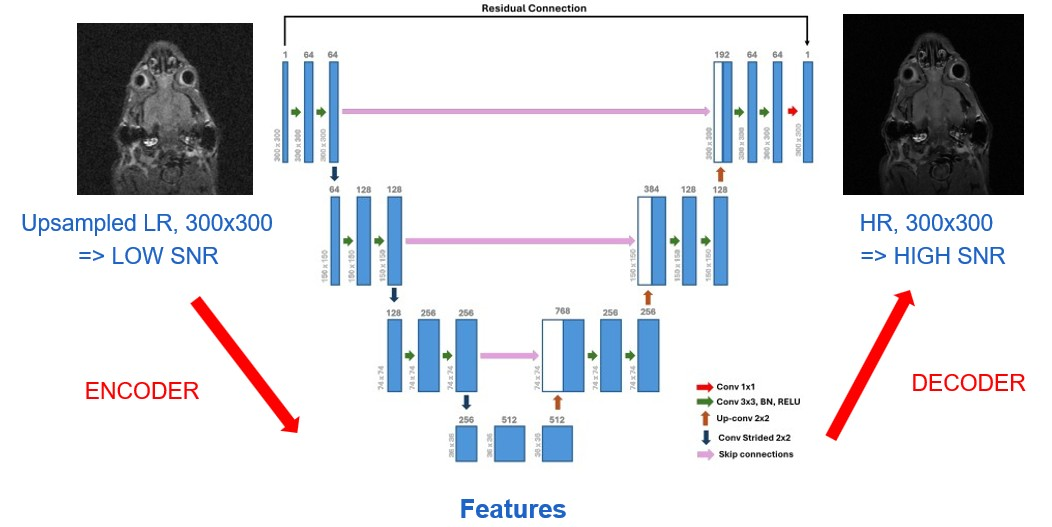
\includegraphics[width=0.5\linewidth]{U-Net.jpg}
    \caption{U-Net architecture.}
    \label{fig:U-Net}
\end{figure}





\subsection{Anchored Path Diffusion Denoising Model (APDDM)}
To complement the direct image-to-image denoising approach, discussed in the previous section, a second model was implemented, the Anchored Path Diffusion Denoising Model (APDDM). This model is a diffusion based framework designed specifically for paired high and low SNR images. In this case the high-resolution (12-minute) scans and the low-resolution (1-minute) scan. Unlike conventional denoising diffusion models that corrupt clean images with artificial Gaussian noise, APDDM uses the actual low SNR image as the endpoint, allowing the model to incorporate real noise from the dataset into the forward process. 

\subsubsection{Forward Diffusion Process}
The forward process defines a stochastic path that gradually transforms the clean image $x_0$ into a noisy version $x_T$, with the endpoint distribution anchored around the real noisy scan $x_t^*$. 
This is achieved using a Markov chain defined by:

\begin{equation}\label{eq:Markov chain}
x_t=q(x_{t-1})=x_{t-1}+\frac{1}{T}\cdot R+f(t)\cdot \hat{\epsilon}, t=1,2,...,T
\end{equation}
\begin{itemize}
    \item $R=x_T^*-x_0$ : the residual between 2 paired images
    \item $\hat{\epsilon} $: noise sampled from empirical residuals
    \item $f(t)=4 \cdot \frac{t}{T} \cdot (1-\frac{t}{T})$ : bell-shaped envelope that controls the noise size
    \item $T$ : the total number of diffusion steps
\end{itemize}


The approach guarantees that the endpoint of the forward diffusion $x_t$ is close to the true low-SNR image $x_t^*$. 
By anchoring the path to $x_t^*$, the model maintains connected to the real noise present in the dataset. 
Additionally the variance in the diffusion path is fully controllable via the envelope function $f(t)$ and the scaling of the noise term $\hat{\epsilon} $, allowing adjustments of how much randomness is introduced. 
This concept is illustrated in Figure \ref{fig:forward APDDM}. The forward diffusion path (indicated in orange) gradually moves from the high-SNR image $x_0$ toward a distribution centered around the noise image $x_T^*$, with each step adding increasing amount of noise. 
The shape of the blue curve represents the variance of the distribution of noise.

\begin{figure}[H]
    \centering
    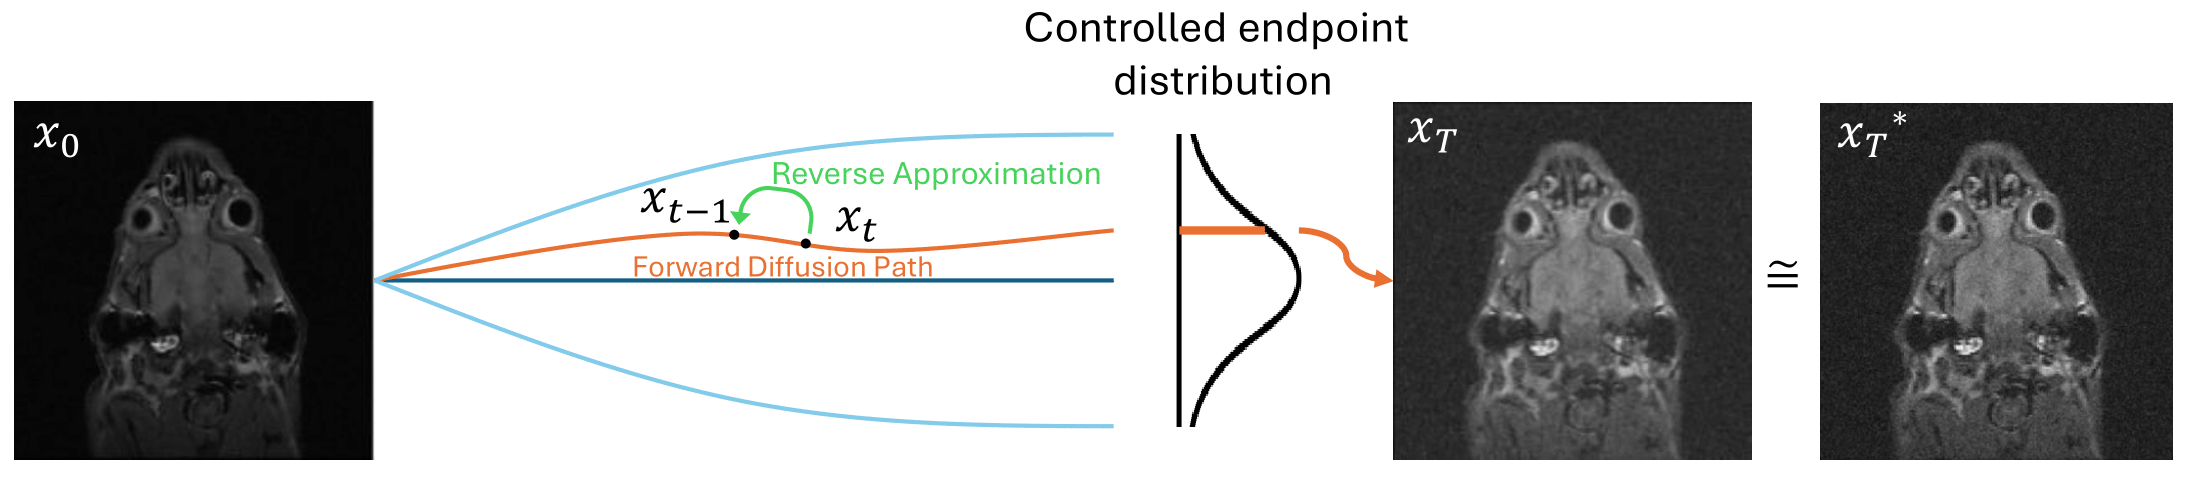
\includegraphics[width=1\linewidth]{forward APDDM.png}
    \caption{forward diffusion APDDM.}
    \label{fig:forward APDDM}
\end{figure}


\subsubsection{Reverse Process and Training}
To reconstruct $x0$ from any intermediate $x_t$, a U-Net model $r_{theta}$ is trained to predict the added noise. 
The predicted noise is then subtracted to obtain an estimate of $\hat{x_0}$, adn training is performed using mean squared error loss: 
\begin{equation}\label{eq:Markov chain}
    \hat{x_0}=x_t-f(t) \cdot r_{\theta}(x_t,\frac{t}{T})
\end{equation}
\begin{equation}
    \mathcal{L}=\|x_0-\hat{x_0}\|^2
\end{equation}
The network does not need to generate high-quality images from scrath but only needs to estimate the noise added from the forward process. 
Figure \ref{fig:APDDM} shows the training strategy. The clean image $x_0$ is transformed into $x_t$ via forward diffusion and the network is trained to reverse this transformation by removing predicted noise and minimizing the loss. 
This setup allows the network to focus on denoising realistic degraded images, guided by noise from the data.

\begin{figure}[H]
    \centering
    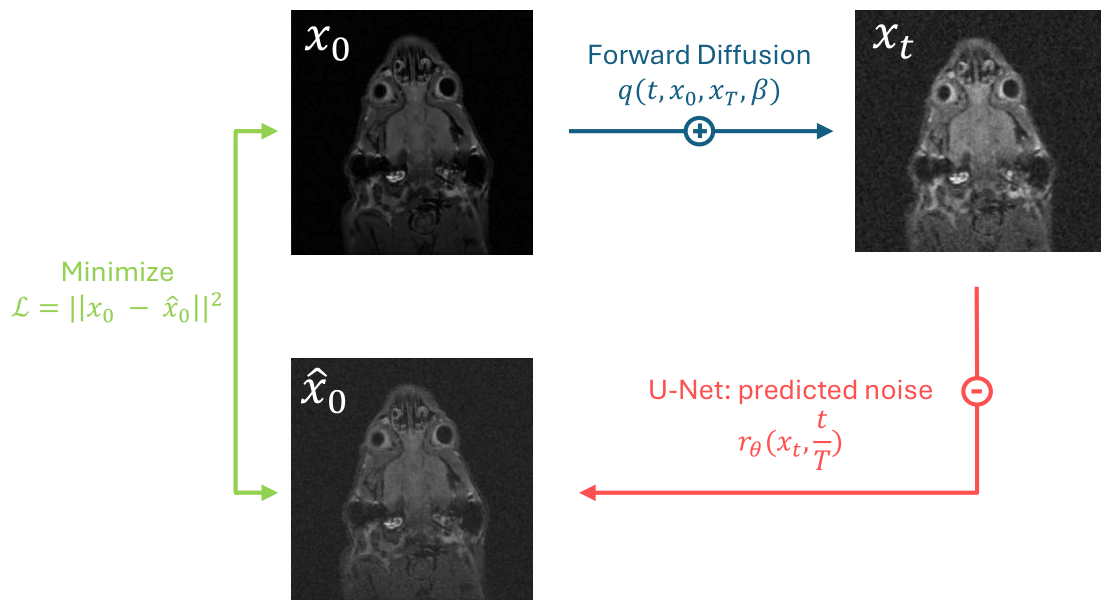
\includegraphics[width=1\linewidth]{full APDDM .png}
    \caption{training overview of APDDM.}
    \label{fig:APDDM}
\end{figure}

\subsubsection{Integration}
APDDM is particularly well suited for our micro-MRI dataset, where paired scans with varying SNR levels are available. 
By using real residuals between the paired images as noise sample, the forward process creates realistic, data-driven noisy versions of the high-resolution images. 
This ensures that the denoising task is meaningful and well-aligned with the expected variation in practice. 
Furthermore, the ability to modulate noise strength and variance offers great control over training difficulty. 
As an example, increasing noise allows for more challenging samples, improving the model's robustness to varying noise levels in unseen data. 
Overall, APDDM offers a highly customizable framework for modeling noise in paired data and provides a strong foundation for future extensions. 
A more mathematical approach can be found in \ref{appendix:Mathematics APDDM}

\subsection{Trained hyperparameters}

To get the best results for the deep learning model for micro MRI image denoising and super-resolution, the hyperparameters need to be fine-tuned. 
In this case Optuna was used to perform automated hyperparameter tuning. 
Giving the number of components and interactions within the model, manual tuning would be inefficient and inconsistent. 
Therefore, an open-source optimization software, such as Optuna, was used. 

At the core of Optuna is the concept of a study, this manages a collection of trials. 
Each trial corresponds to the training of the model with a specific set of hyperparameters. 
The performance metrics are recorded after each trial, for example a validation loss. These metrics are used as a guide for the search. 
A built-in sampler selects new parameter values to explore, while a pruners stops trials early if the model is clearly not improving. 
This combination is especially helpful to reduce the number of trainings that need to be run, this saves computational resources. 

One of the advantages of Optuna is its define-by-run approach \cite{10.1145/3292500.3330701}. 
This means that instead of predefining the entire parameter space before the optimization, the search space is defined dynamically while being executed. 
This gives more flexibility especially in cases where certain parameters are only relevant under specific conditions. 
Instead of testing all combinations blindly, Optuna can selectively explore subsets of the parameter space based on earlier decisions within the same trial. 
The avoidance of meaningless testing makes the optimizations process  more efficient. 

Overall Optuna played a key role in helping reach a well-performing model more efficiently, and ensured that our final configuration was based on data-driven search rather than trial and error.

The following parameters were included in our optimization process:

\subsubsection{Early stopping}
To avoid excessive training of the model, the Early Stopping is used. 
This parameter is defined as 'no update since' value, which the user must set. 
If this number is set too low, the model may avoid overfitting but could also stop training prematurely. 
On the other hand, setting the value too high may result in an ineffective use of the Early Stopping. 
In this project, at least 10 epochs will be ran. If there is no improvement during 6 epochs, the program will be stopped.

\subsubsection{Optimizer}
The optimizer plays a crucial role in fine-tuning the model's weights during training to minimize the loss function. 
Different methods can be used, each with its own advantages and disadvantages. 
In this project four different optimizers will be tested: torch.optim.Adam, torch.optim.AdamW, torch.optim.SGD and torch.optim.RMSprop. 
Adam combines the benefits of momentum and adaptive learning rates.  
One of its limitations is the way it incorporates L2 regularization directly into the gradient update, which can sometimes negatively affect the performance. 
In contrast, AdamW decouples weight decay from the gradient update, applying it separately after the parameter update, which provides a more effective approach \cite{pykes-2021}.
Stochast gradient descent (SGD) updates the model's parameteres based on the gradient loss function. 
Unlike Adam, it uses a fixed learning rate and does not estimate moments of the gradients \cite{massed-compute-2025}.
RMSprop is another gradient-based optimization algorithm. 
It uses an adaptive learning rate instead of treating the learning rate as a hyperparameter, which results in a change of learning rate over time. 
This can result in faster convergence \cite{sanghvirajit-2025}.

\subsubsection{Scheduler} \label{subsec:Scheduler}
The scheduler adjust the learning rate during training according to the strategy that is predefined. 
The following schedulers will be tested: \texttt{ExponentialLR}, \texttt{StepLR}, and \texttt{ReduceLROnPlateau} from the PyTorch \texttt{torch.optim.lr\_scheduler} module.

The ExponentialLR divides the learning rate every epoch by the same factor $\Gamma$. 
As a result, the learning rate decreases abruptly during the first epochs and then gradually stabilizes, approaching zero over time. 
StepLR is similar to ExponentialLR. It also decays the learning rate by gamma. However, the key difference is that this decay occurs only every N epochs. 
This leads to more gradual and less frequent reductions in the learning rate compared to ExponentialLR. 
This difference can be seen in \ref{eq:1} and \ref{eq:2}.
Another scheduler is ReduceLROnPlateau. Unlike the others, it adapts the learning rate based on the performance of a specified metric. 
This algorithm decreases the learning rate when the specified metrics stops improving for longer than the patience number allows. 
So, the learning rate is kept constant as long as the metric improves quantity. 
When the learning rate is reduced, the results stagnate \cite{unknown-author-no-date3} \cite{isbhargav-2020}. 

\begin{equation}\label{eq:1}
lr_{\text{epoch ExponentialLR}} = \Gamma \times lr_{\text{epoch}-1}
\end{equation}

\begin{equation}\label{eq:2}
\resizebox{1.\hsize}{!}{$
lr_{\text{epoch}} =
\begin{cases}
\Gamma \times lr_{\text{epoch}-1}, & \text{if } \text{epoch} \bmod \text{step\_size} = 0 \\
lr_{\text{epoch}-1}, & \text{otherwise}
\end{cases}
$}
\end{equation}

\subsubsection{Learning rate decay}
The learning rate decay will decrease the learning rate when the training progresses and becomes more stable. 
It is used in the Scheduler algorithms as the step size (see \ref{subsec:Scheduler}). 
Here, the learning rate decay of 0.1, 0.,3 and 0.5 is tested.

\subsubsection{Features main and features skip}
To decide which main features are used, different powers of $2$ were used. 
For every component of features\_main matrix, a different power can be chosen. 
The next elements of the matrix will contain the next powers of $2$. It can be chosen how many elements will be used in the matrix. 
For the features\_skip, the same matrix as features main was chosen with the last element deleted. 
We conducted experiments using a setup where one value was selected from each of the defined categories. 
Specifically, features\_main\_1 was chosen from [32, 64, 128], features\_main\_2 from [64, 128, 256], and features\_main\_3 from [128, 256, 512]. 
This approach allowed us to systematically explore different combinations of feature sizes and assess their impact on the model's performance.

\subsubsection{Upsampling method}
The upsampling method is the process by which the resolution of an image is increased while minimizing the loss in image quality. 
The goal is to increase the number of rows and/or columns of the image. Several methods are available, including nearest, linear, bilinear, trilinear, and bicubic interpolation, as implemented in torch.nn.Upsample.
The nearest neighbor interpolation is the simplest approach. 
Each pixel of the upscaled image is assigned the value of its nearest neighbor in the original image. 
This method is fast and simple, but can produce pixelated images.
The linear interpolation calculates the new pixel value by taking a weighted average of the two nearest pixels along a single axis. 
The bilinear interpolation calculates a weighted average of the four nearest neighbors' pixel values in the original image. 
It uses linear functions and a 2x2 pixel grid. 
The trilinear interpolation is used in 3D images. 
The interpolation is first performed linearly along one axis, followed by linear interpolation along the second and third axes. 
The linear, bilinear and trilinear methods result in smoother images than the nearest method.
Bicubic interpolation is more advanced. This interpolation method first identifies the nearest 4x4 grid of pixels surrounding that point that needs to be interpolated. 
Then, it calculates the cubic polynomials that best fit the pixel values in the grid. 
After that the pixel intensity is estimated at the target position. 
It is an effective method for high-quality upscaling because it preserves details and reduces artifacts \cite{amanrao-2023} \cite{unknown-author-2025}.

\subsubsection{Downsampling method}
The downsampling method is important in the encoder and tells how the images will be reduced. Different methods were considered. 
Maxpooling selects the maximum value from each patch in the feature map, preserving the most prominent features while reducing spatial dimensions. 
This concept can be observed in Figure ~\ref{fig:maxpool} \cite{dhanushkumar-2023}.
Another approach is Meanpooling. Instead of taking the prominent feature, this method averages the values within a patch, offering a smoother downsampling method. 
In Figure ~\ref{fig:meanpool} the concept of meanpool can be seen.
The last method, that is observed in this project, is convStrided. The principle can be seen in Figure ~\ref{fig:convStrided}. 
First, the image is upsampled to increase its resolution (if necessary). 
Next, the convolution is applied with a larger stride. 
The strides controls how much the filter moves across the feature map during the convolution process. 
When the the stride is greater than 1, the convolution operation skip some of the pixel, which results in an effective method to reduce the size of the feature map \cite{unknown-author-no-date2}.
Each of these methods reduce the size of the feature map but with different strategies.


\begin{figure}
    \centering
    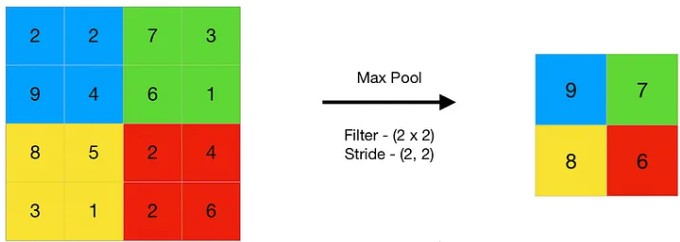
\includegraphics[width=1\linewidth]{Maxpool.jpg}
    \caption{Downsampling - Maxpool}
    \label{fig:maxpool}
\end{figure}

\begin{figure}
    \centering
    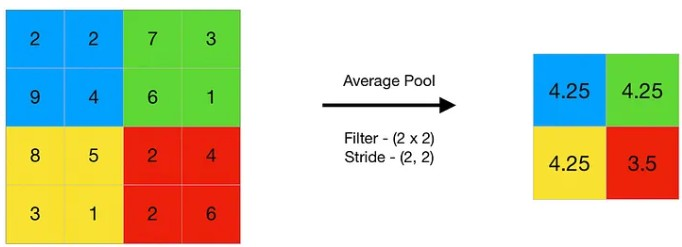
\includegraphics[width=1\linewidth]{Meanpool.jpg}
    \caption{Downsampling - Meanpool}
    \label{fig:meanpool}
\end{figure}

\begin{figure}
    \centering
    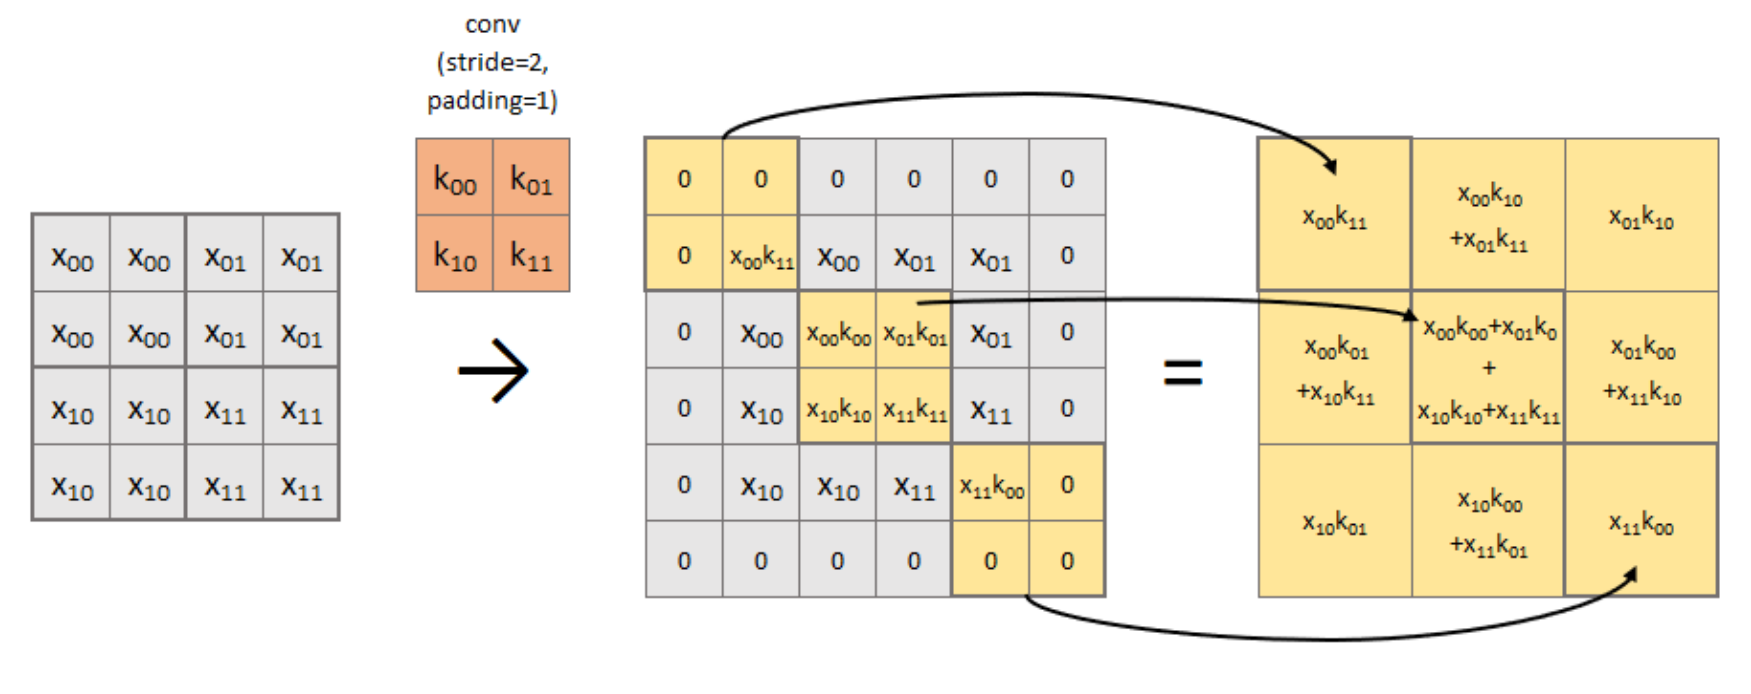
\includegraphics[width=1\linewidth]{ConvStrided_new.png}
    \caption{Downsampling - convStrided}
    \label{fig:convStrided}
\end{figure}

\subsubsection{Learning rate}
The pace in which the weights are updates during training depends on the learning rate. 
A learning rate value which is too high can lead to instability and poor convergence, while a value too low might slow down the training of the model  as can be seen on Figure \ref{fig:Learnrate} or it can even get stuck in a local minima \cite{jordan_2018_setting}. 
Optuna was used to search across a continuous range of values [1E-2, 1E-6] to find the optimal balance between convergence and stability.

\begin{figure}
    \centering
    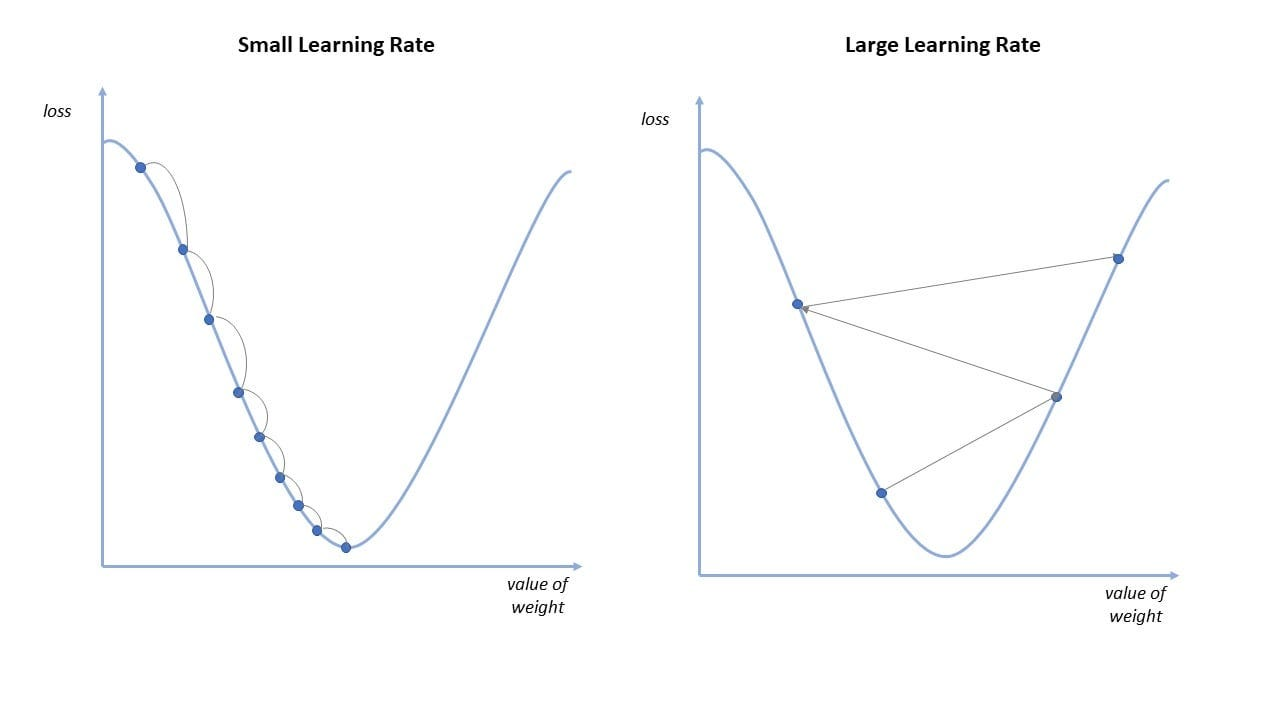
\includegraphics[width=1\linewidth]{Learn rate.jpg}
    \caption{Comparison of different learning rates}
    \label{fig:Learnrate}
\end{figure}

\subsubsection{Loss function}
The loss function defines how well our model is performing by evaluating the prediction against the target images. 
It guides the process by providing a measure of error which then can be minimized during training. 
3 loss function were tested: Mean Squared Error (MSE) , Mean Absolute Error (MAE) and a hybrid loss. 
MSE penalizes the squared difference between the predicted and true pixel values. 
This loss function penalizes large errors more severely because the errors are squared. 
This method is effective for achieving high numerical accuracy but can lead to overly smooth outputs with less fine structural detail.
MAE computes the average of the absolute differences between predicted and true pixel values. 
This method preserves edges and sharper transitions better than MSE but it is less sensitive to small errors and can converge more slowly \cite{anderson_2023_loss}.
The last option, the hybrid loss, is a custom-defined loss which combines mean squared error (MSE) and structural similarity index (SSIM).
\begin{equation}\label{eq:3}
\mathcal{L}_{\text{hybrid}} = \alpha \cdot \mathcal{L}_{\text{MSE}} + (1 - \alpha) \cdot (1 - \text{SSIM})
\end{equation}
\begin{itemize}
    \item $\alpha \in [0, 1]$ controls the balance between the two components,
    \item $\mathcal{L}_{\text{MSE}}$ measures the average pixel-wise error between the predicted and ground truth images,
    \item $\text{SSIM}$ evaluates perceptual similarity.
\end{itemize}
MSE helps preserve pixel-wise fidelity while SSIM ensures structural integrity of the image, which is crucial in medical contexts. 
Optuna was used to choose the type of loss function to apply and, in the case of the hybrid loss, to optimize the value of alpha. 
This allowed the model to adaptively prioritize pixel accuracy versus perceptual quality. 

\subsubsection{Activation function}
Activation functions introduce a non-linearity into the network. This allows complex mapping between inputs and outputs. 
Without an activation function the network would behave like a linear system and would not be able to model intricate relationships suchs as edges and contrast. 
Different options were tested such as ReLU,  LeakyReLU and ELU. Each of these options come with their own set of advantages and difficulties. 
ReLU (Rectified Linear Unit) is most commonly used as an activation function because of its simplicity and computational efficiency. 
This function \ref{eq:4} returns the positive inputs directly and zero if negative. One of the limitations is a phenomena called 'dying neurons',  if a neuron only receives negative inputs, it will always output zero and stop learning.
LeakyReLU adresses this problem by allowing small negative outputs. This function \ref{eq:5} helps keeps neurons active and keeping them active. 
This technique keeps the simplicity or ReLU while improving stability. 
ELU is similar to LeakyReLU in the idea of keeping negative ouputs, but in this case with a smooth exponential curve \ref{eq:6}  instead of a constant curve. 
Finally PReLU (Parametric ReLU) also starts from LeakyReLU but in this case the negative slope is a learnable parameter and not a fixed value. 
This lets the model adapt the activation function in training leading to potentially better performance. 
However it does introduce an extra parameter increasing computational cost \cite{bharatiya_2019_comprehensive}.

\begin{equation}\label{eq:4}
    f(x)_{ReLU} = \max(0, x)
\end{equation}

\begin{equation}\label{eq:5}
f(x)_{LeakyReLU} = 
\begin{cases}
x & \text{if } x \geq 0 \\
\beta x & \text{if } x < 0
\end{cases}
\end{equation}

\begin{equation}\label{eq:6}
f(x)_{ELU} = 
\begin{cases}
x & \text{if } x \geq 0 \\
\alpha (e^x - 1) & \text{if } x < 0
\end{cases}
\end{equation}


\begin{equation}\label{eq:7}
f(x)_{PReLU} = 
\begin{cases}
x & \text{if } x \geq 0 \\
a x & \text{if } x < 0
\end{cases}
\end{equation}

\subsubsection{Batch size}
Batch size defines how many training samples are used to calculate the gradient before the model updated the weights. 
A larger batch size gives a more gradient estimate which can speed up training, but it requires large memory and can lead to worse generalization. 
While a small batch size is more noisy in gradient updates which can escape local minima but also may lead to slow convergence. 

\subsubsection{Residual learning}
With residual learning instead of predicting the final high-resolution images the model learns the difference between the low- and high-resolution, this is called the residual. 
After training the residual is added back onto the input image to produce the final image. This method has its advantages. 
Learning the missing information is often faster and easier than predicting the entire image. This can lead to faster and better convergence. 
In this project residual learning is an optional feature. Optuna was used to explore if enabling led to better performance.

\subsubsection{Number of epochs}
The number of epochs defines how many times the model goes through the entire training dataset. 
While this is not a traditional hyperparameter it still has a role in the performance of the model. 
Too few epochs can lead to underfitting, the model has not learned enough (especially with smaller datasets). 
Too many can lead to overfitting, a phenomenon where the model memorizes the training data and performs poorly on unseen samples. 

\section{Validation methods}
In this section, the used validation methods are described. All the methods check the performance of the model. 

\subsection{Mean squared error}
The mean squared error (MSE) measures the amount of error in statistical models by taking the average squared difference between the observed and predicted values. 
If there is no error, the MSE will become zero. Formula \ref{eq:MSE} can be used to calculate the MSE: 

\begin{equation}\label{eq:MSE}
    \text{MSE} = \frac{1}{x \cdot y} \sum_{i=0}^{x-1} \sum_{j=0}^{y-1} \left( S(i, j) - \hat{S}(i, j) \right)^2
\end{equation}

Here, S(i, j) is the observed value, and $\hat{S}(i, j)$  is the corresponding predicted value. 
X represents the number of pixels in a row and y denotes the number of pixels in a column. \cite{mseJim}

The MSE was calculated for the high resolution and the result of the deep learning model. After these calculations the ratio is taken.

\subsection{Structural similarity index measure}
Since MSE can't account for structural composition, structural similarity index measure (SSIM) is used. 
SSIM assesses the structural similarity between two images by considering luminance, contrast, and structure. 
It can be used to evaluate the quality of the deep learning model compared to the pre-scanned high resolution images. 
This evaluation metric is especially useful in medical image applications.

\begin{equation}\label{eq:SSIM}
\text{SSIM}(A, B) = \frac{(2 \cdot \mu_A \cdot \mu_B + c_1)(2 \cdot \sigma_{AB} + c_2)}{(\mu_A^2 + \mu_B^2 + c_1)(\sigma_A^2 + \sigma_B^2 + c_2)}
\end{equation}

\begin{itemize}
    \item $\mu_a,\mu_b$ : mean intensities of images A and B
    \item $\sigma_A^2, \sigma_B^2$ :variances
    \item $\sigma_{AB}$ : covariances
    \item $c_1,c_2$ : 2 variables which stabilize the division (both are typically small values)
\end{itemize}

 The SSIM value is typically in the range of [0,1], where a value closer to 0 represents lower levels of image quality and values nearer to 1 represents higher levels of quality. \cite{dosselmann-2009}

 \subsection{Contrast-to-noise ratio}
 Contrast-to-noise ratio (CNR) is a metric that evaluates the quality of an image by measuring how well a region of interest (for example, liver) can be distinguished from the surrounding background.
\begin{equation}\label{CNR}
\text{CNR}=\frac{\mu_{ROI}-\mu_b}{\sigma_b}
\end{equation}

$\mu_{ROI}$ is the mean of the region of interest, $\mu_b$ is the mean of the background and $\sigma_b$ is the noise in the background.
A higher CNR value indicates better differentiation of the region of interest from its background.

\subsection{Visual comparison}
In addition to quantitative measurements, a visual inspection can also be done to evaluate the quality of the reconstructed images. 
The visual comparision will compare the residuals of high-resolution and low-resolution images to the residuals of high-resolution and deep-learning images. 
Ideally the residual of high-resolution and deep-learning images should be close to zero in most regions, indicating an accurate reconstruction. 

\section{Results}
\subsection{First results}
First the model was runned on the hpc to check if everything went correctly. 
With this first run, the pre-processing steps could be verified and the first results could be observed. 
The training was done on the accelgor cluster. 
The 11th epoch was the best one, as can be observed in Figure \ref{fig:first_loss}.
In the best epoch the loss of the training is equal to 0.481, while the one of the validation equals 0.426.

\begin{figure}
    \centering
    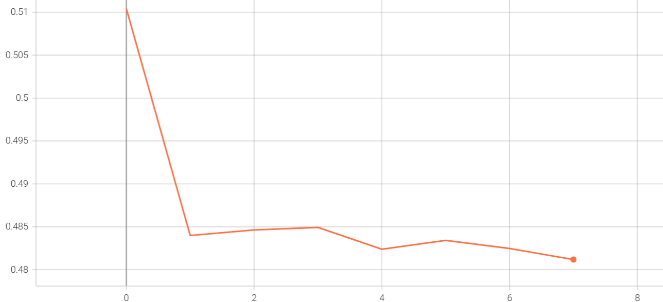
\includegraphics[width=1\linewidth]{First_results_loss.png}
    \caption{Visual representation of the loss function over different epochs. ER STAAN GEEN ASSEN OP DEZE FIGUUR!!!!!!}
    \label{fig:first_loss}
\end{figure}

In this script the training, validation and test mice were defined. A detailed overview can be found in Table \ref{tab:mouse_distribution}.
The features\_main were set to [64, 128, 256], with corresponding features\_skip values of [64, 128]. 
Meanpooling was used for downsampling, and upconv was applied for the upsampling steps. 
The activation function was ReLU, and residual connections were enabled True.
The model was trained with a batch size of 32 and a learning rate of 0.0001. Training was conducted over 200 epochs. 
The RMSprop optimizer was used along with an ReduceLROnPlateau scheduler. MSE was employed as the loss function.
These hyperparameters were chosen based on knowledge and guessing what the best one would be.

In Figure \ref{fig:first_sagittal}, Figure \ref{fig:first_transax} and Figure \ref{fig:first_coronal} the results can be observed, where each is an example of the training mice. 
Since the output gave not all images back, Figure \ref{fig:first_coronal} is a result of the 13th epoch.
Each image depicts another plane of the mouse. Also, images of the test mice can be found in Appendix \ref{Appendix: Figures Results}

\begin{figure*}
    \centering
    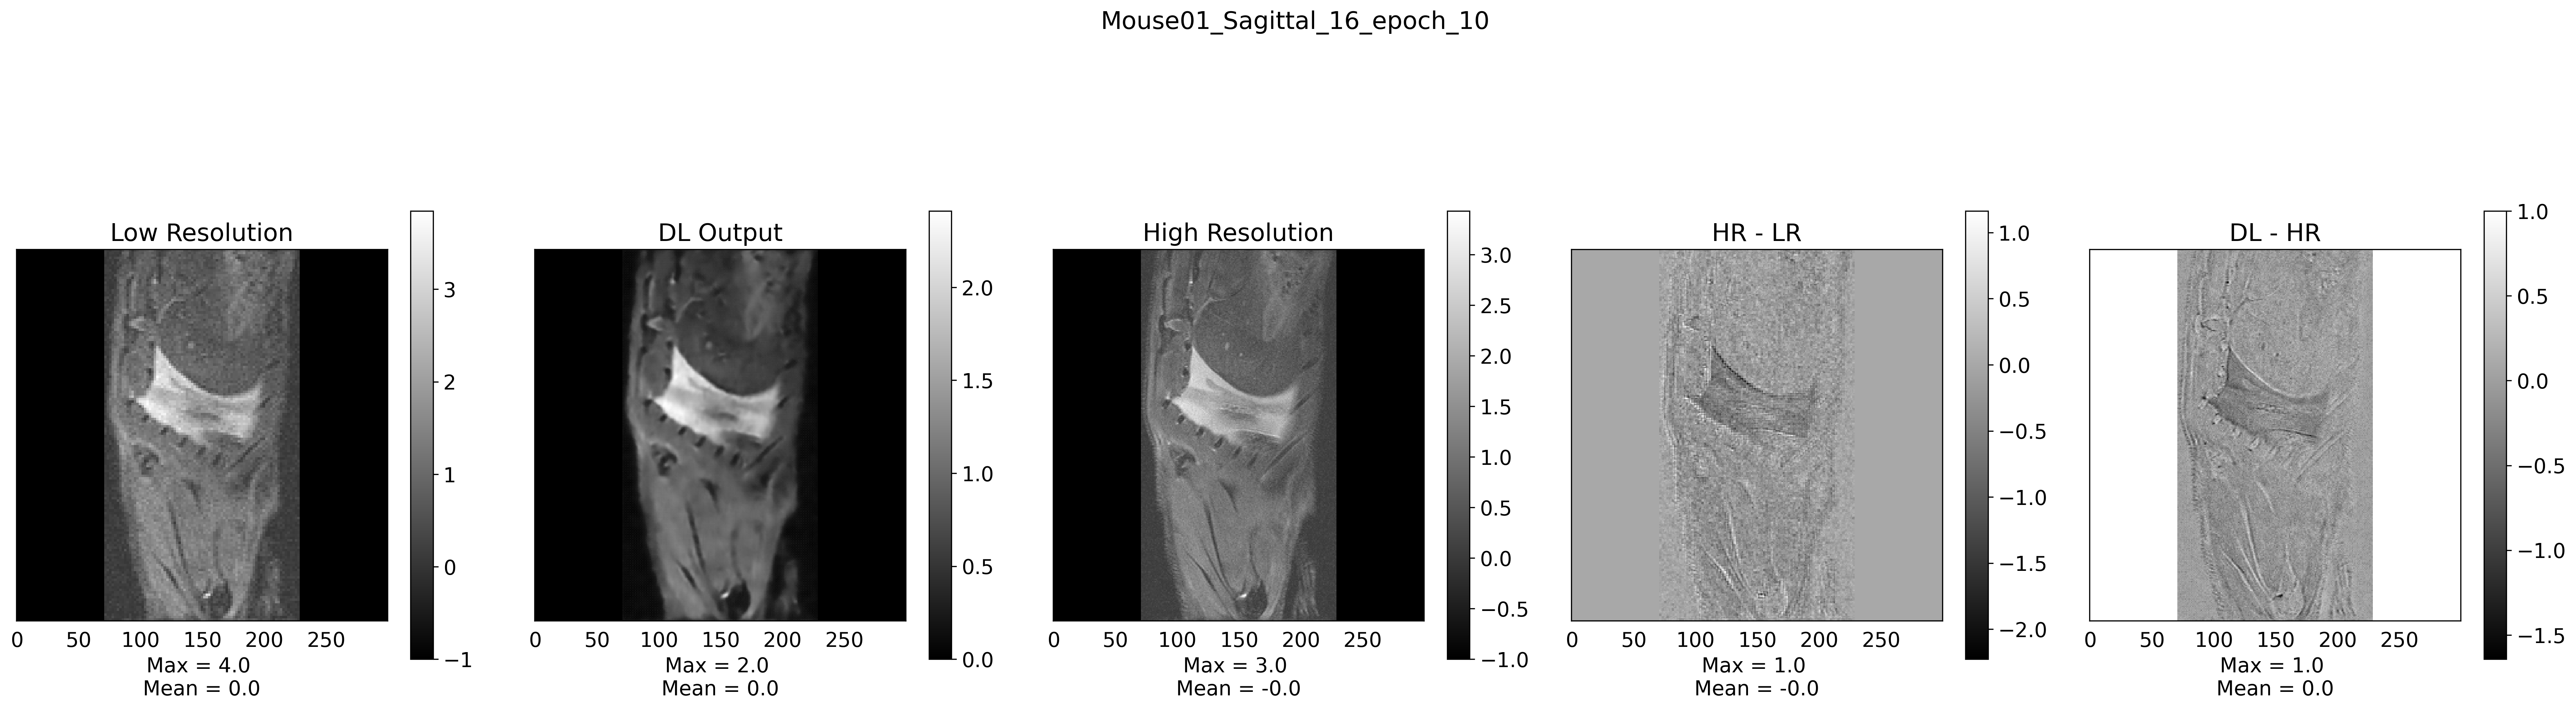
\includegraphics[width=1\linewidth]{Mouse01_Sagittal_16_epoch_10.png}
    \caption{First results of mouse 1 (training) sagittal plane slice 16 after 11th epoch.}
    \label{fig:first_sagittal}
\end{figure*}

\begin{figure*}
    \centering
    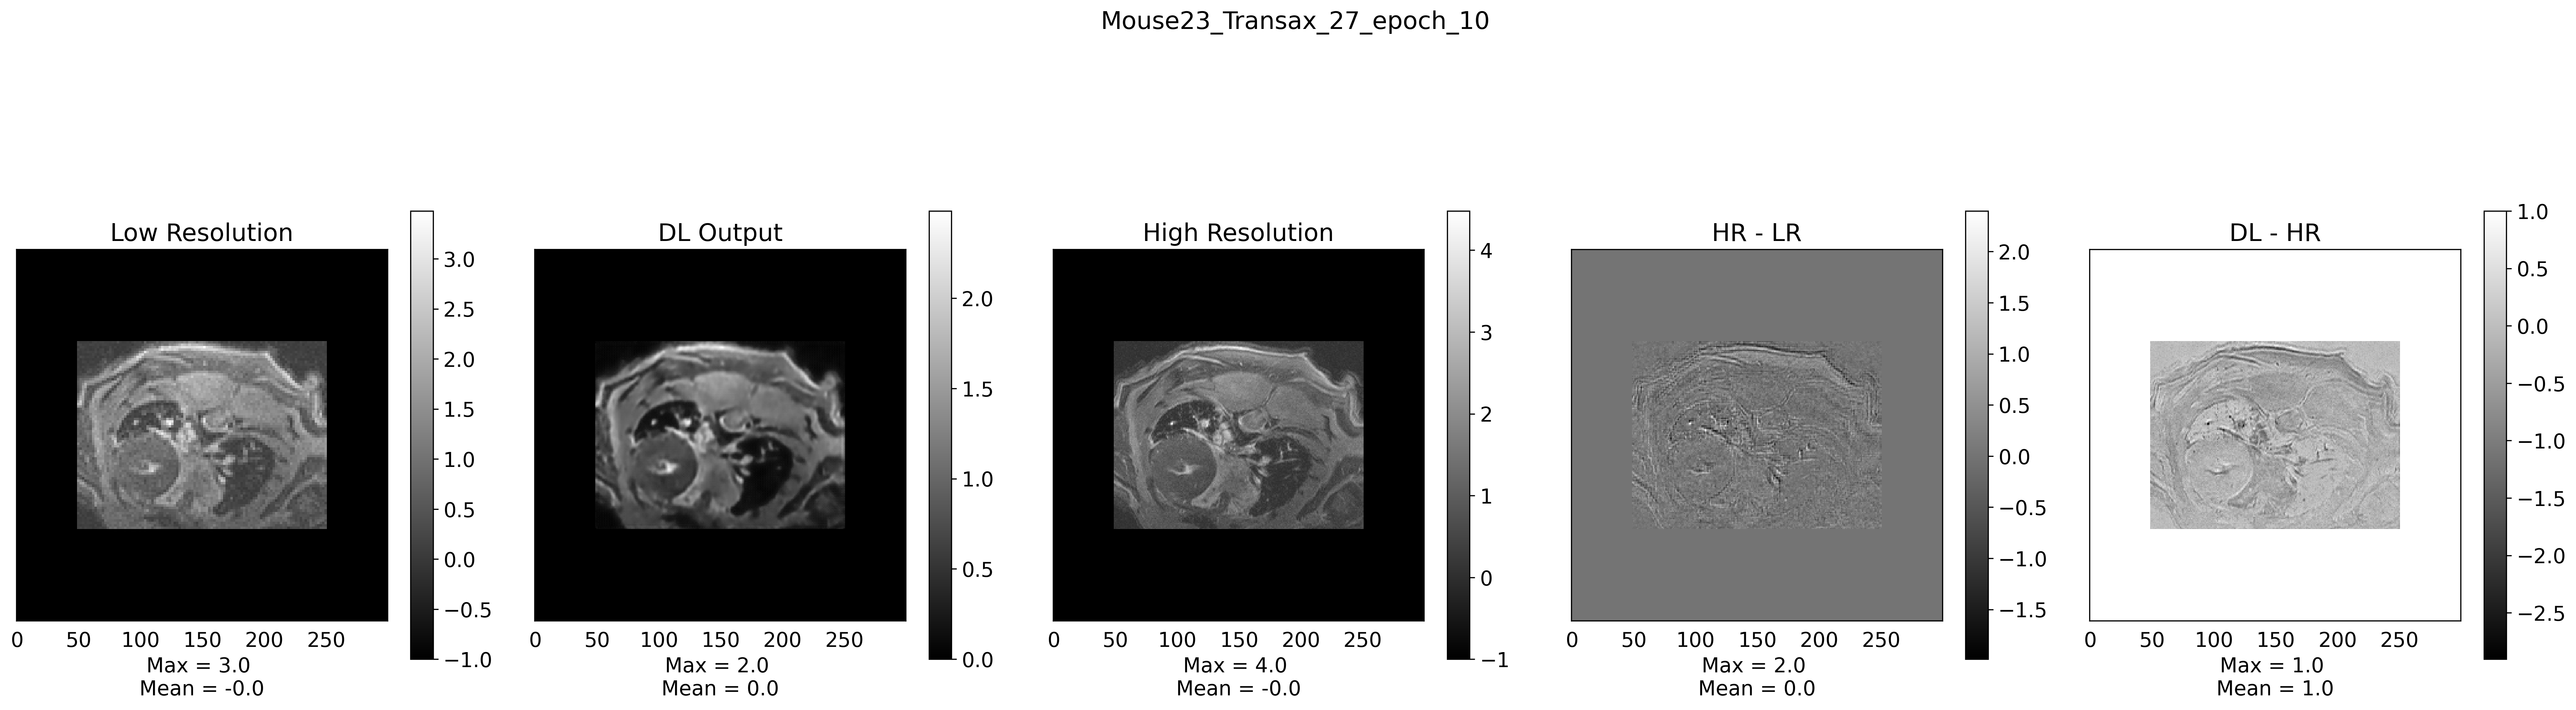
\includegraphics[width=1\linewidth]{Mouse23_Transax_27_epoch_10.png}
    \caption{First results of mouse 23 (training) transaxial plane slice 27 after 11th epoch.}
    \label{fig:first_transax}
\end{figure*}

\begin{figure*}
    \centering
    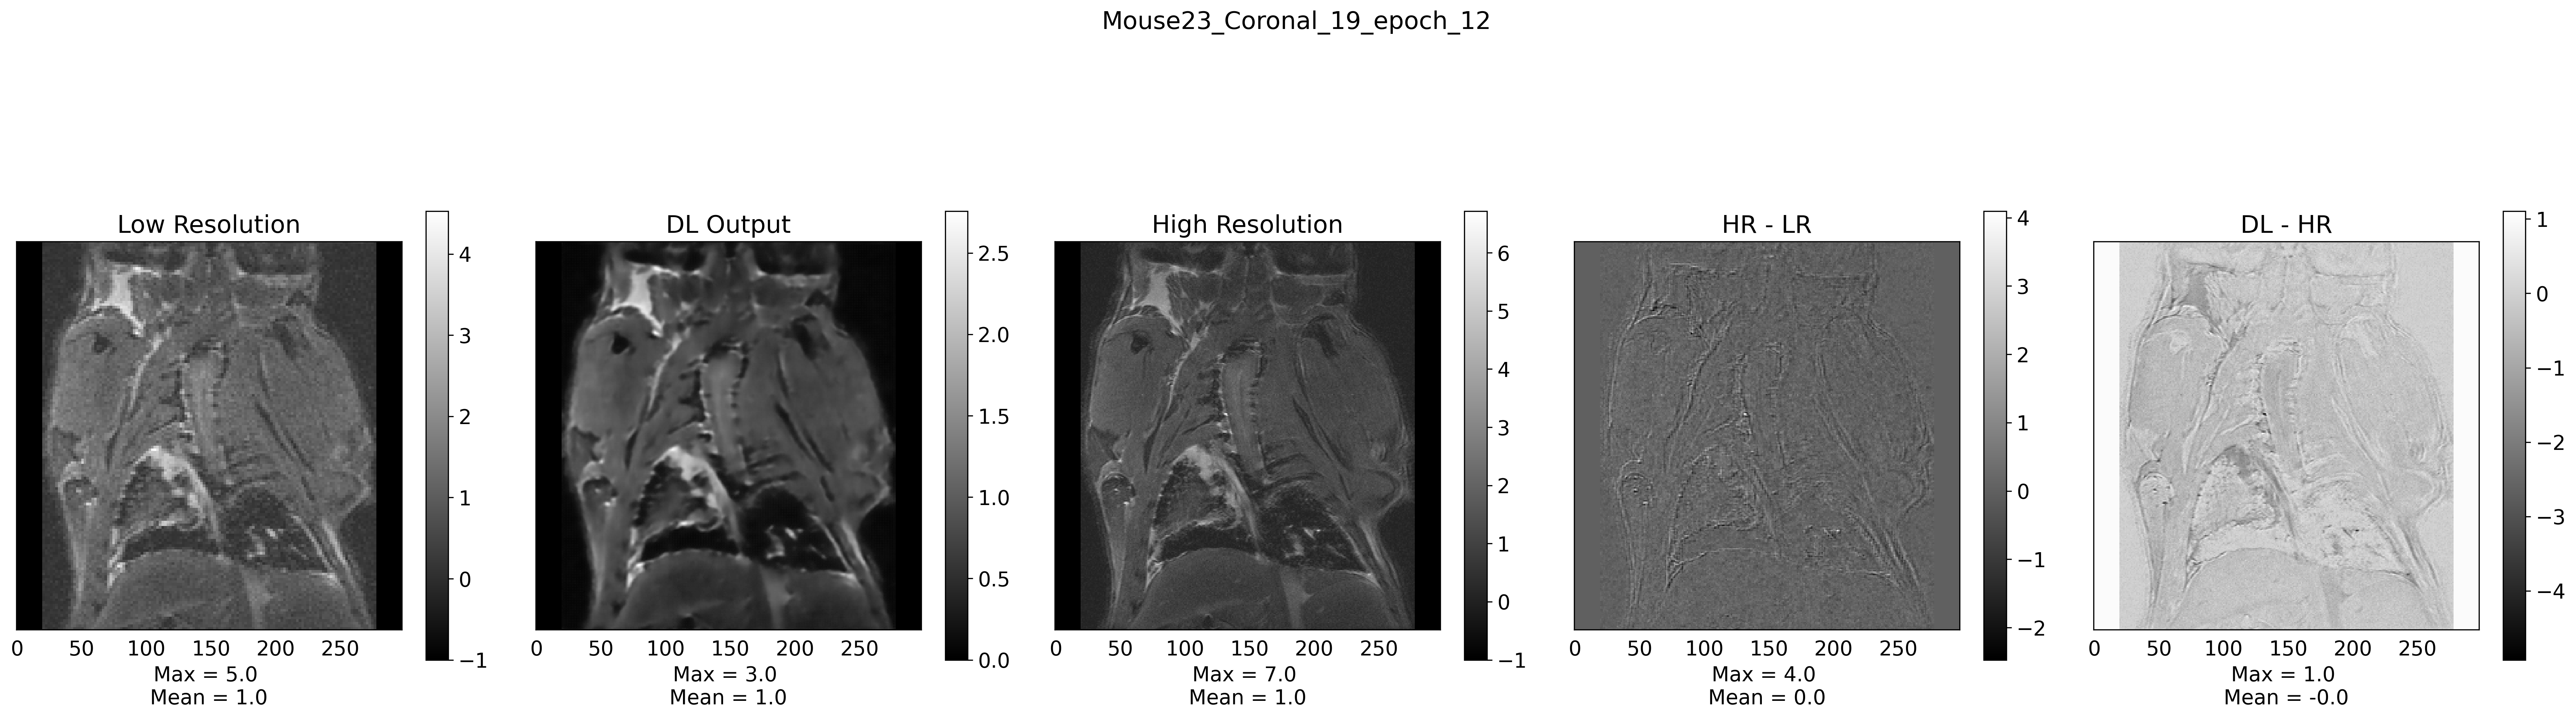
\includegraphics[width=1\linewidth]{Mouse23_Coronal_19_epoch_12.png}
    \caption{First results of mouse 23 (training) coronal plane slice 19 after 13th epoch.}
    \label{fig:first_coronal}
\end{figure*}


\subsection{Trained hyperparameters}
\subsubsection{First optimization}
The first hyperparameter optimization process conducted with Optuna evaluated multiple architertural and training configurations for a U-Net based model. 
Trail 54 emerges as the best-performing configuration, achieving a validation MSE of 0.0984. 
This model uses a structure with convolutional feature depths of 128, 256, 256 for the main layers. 
Downsampling was performed using strided convolutions and upsampling with transposed convolutions. 
The ReLU activation function was used and residual output connections were disabled. 
Optimization was done using the RMSprop algorithm with initial learning rate of 0.004112 in combination with the ReduceLROnPlateau learning rate scheduler. 
The model was trained using a hybrid loss function that combines MSE and SSIM with the weighting controlled by a parameter $\alpha=0.3$.
This combination of hyperparameters resulted in the lowest validation MSE across all evaluated trials, indicating strong performance in reconstructing high-resolution images. 

\subsubsection{Disclaimer}
It was later discovered that the optimization function was not working as intended and this was due to 2 reasons.
First the custom loss function did not function correctly. Second of all Optuna was run only on transaxial slices and only on 2 mice. 
As a result, the hyperparameters and validation metrics do not generalize to the full dataset. 

To address this problem, a second Optuna optimization was run with corrected loss function and a full dataset. 
The revised optimization yielded different best performing parameters. 

\subsubsection{Second optimization}


\subsection{Results after hyperparameter training}


\begin{table}[h]
    \centering
    \resizebox{0.97\linewidth}{!}{  % Schaal de tabel tot 80% van de kolombreedte
    \begin{tabular}{l|c|c|c}
    \toprule
     & \textbf{Training} & \textbf{Validation}& \textbf{Testing} \\
    \hline
    \midrule
    Mouse & \makecell{1, 2, 3, 4, 5, 8 \\ 9, 11, 12, 13, 14, 15 \\ 17, 18, 19, 20, 21, 23} 
              & \makecell{6, 10}
              & \makecell{7, 16, 22} \\
    \bottomrule
    \end{tabular}
    }
    \caption{\label{tab:mouse_distribution} Mouse distribution across training, validation, and testing sets.}
    \end{table}

    

\subsection{APDDM}

\subsection{Validation}

\section{Discussion}
\subsection{First results}
After obtaining the first results, a visual validation was made. At first sight, the results were very promising. 
Looking at the Figure \ref{fig:transax1_first} and Figure \ref{fig:transax2_first} shows that the deep learning (DL), in the middle, has clearly higher quality and sharper details compared to the low resolution (LR) image at the left side. 
The DL image approaches the high resolution (HR), but still has noise and structures that are not totally visible. 
In Figure \ref{fig:transax1_first}, the maximum intensity of the DL image is the same as that of the LR, which both have an intensity of 5, while the maximum intensity of the HR is higher with an intensity of 6. 
This indicates small intensity bias or scaling difference. 
This is in contrast with Figure \ref{fig:transax2_first} where the maximum intensity (equal to 4) is lower than in the LR and HR images, where the mean value is 5. 
This can be due to the liver that is smeared out and more depicted gray as in both LR and HR scans.
Looking at the edges of the DL images it shows that these are generally more smeared out and less sharp than in the HR images. 
The noise of the LR is reduced with minimal loss of important structural information. 
As said, the results are very promising but there is also room for improvement. The first step in this process is training the hyperparameters. 
An important note to make is that the validation and test set for the first results were not well chosen. 
All the images that were scanned during this project are set as validation, which could lead to bias. 
This will be taken into account when training the model a second time.

\subsection{Trained hyperparameters (work in progress)}
Trial 54 achieved a strong validation MSE of 0.0984. 
Several key hyperparameter choices reflect current best practices in deep learning for medical image restoration, while others diverge in notable ways. 

The feature dimensions were set to 128,256 and 256 across the 3 main layers. 
This progressive increase allows the network to capture abstract and complex image features as spatial resolution decreases. 
The depth of the layers contributed to the model's ability to reconstruct finer details.

ReLU was selected as activation function over other alternatives such as LeakyReLU or ELU. 
While ReLu is prone to "dying neurons", its simplicity, speed and effectiveness in networks make it a robust default choice \cite{relu}. 
The absence of a relatively complex activation function suggests the network did not suffer from gradient issues that would call for alternatives. 
Strided convolution (convStrided) was preferred over pooling for downsampling. 
This aligns with expectations from common CNN practive. 
Strided convolution allows the model to learn how to compress feature maps instead of relying on fixed operations such as meanpooling. 
This learnability likely helped preserve critical structural details. 

Upsampling was performed using transposed convolutions (upconv), as a standard approach that allows the network to recover spatial resolution in a data-driven way. 
Unlike other methods, upconv layers can learn to reintroduce high-frequency detail, making them well suited in this case.

Residual connections were disabled which is an unexpected result which contrasts with many image restoration models that benefit from residual learning. 
However, it can be explained due to the skip connections inherent to U-Net which likely compensated for this. 
This allows effective feature reuse and reduces the need for a global residual link.

The learning rate was set to 0.004113 which is relatively high initial value. This enables faster early convergence. 
The optimization setup combined RMSprop and ReduceLROnPlateau. 
RMSprop adjusts the learning rate for each parameter individually based on the recent history of the gradients \cite{9036442}. 
This helps stabilize updates, especially when gradients vary in scale. 
In parallel, the ReduceLROnPlateau scheduler monitors the validation loss and automatically lowers the global learning rate when improvements slow down. 
Together these tools contribute to faster and more stable convergence, reducing the risk of overshooting or stagnation.

The model was trained using a hybrid loss function that combines both MSE and SSIM, with  $\alpha=0.3$. 
Because of \ref{eq:6} it can be concluded that structural similarity is favored, encouraging the model to preserve structural features over strict pixel accuracy. 
Such a loss is better suited in medical imaging tasks than pure MSE which can lead to overly smooth, less diagnostic outputs \cite{Dastmalchi}. 

The optimization process solely relied on MSE for validation. This decision may introduce some form of metric bias. 
MSE disproportionately penalizes large pixel errors, which often lead to overly smooth outputs. 
In denoising tasks, this can result in models that reduce noise effectively in terms of pixel accuracy but at the cost of signal preservation, leading to a lower signal-to-noise (SNR) in practice. 
MSE is also sensitive to outliers and intensity shifts, while being oblivious to perceptual structure and contrast consistency \cite{1284395}. 
Future work could benefit from using alternative validation metrics, such as SNR or perceptual similarity measures, to better guide model selection and ensure outputs are both quantitatively accurate and visually informative \cite{chavhan2009t2star}. 
Metrics such as LPIPS offer a promising alternative by leveraging deep features that align more closely with human perception and quality \cite{zhang2018unreasonableeffectivenessdeepfeatures}.

\subsection{Results after hyperparameter training}

\subsection{APDDM}

\subsection{Validation}

\section{Conclusion}

\newpage
\onecolumn
\nocite{*}
\begin{thebibliography}{99}

    \bibitem{brown2014magnetic} Brown, R. W., Cheng, Y.-C. N., Haacke, E. M., Thompson, M. R., \& Venkatesan, R. (2014). \textit{Magnetic Resonance Imaging: Physical Principles and Sequence Design}. John Wiley \& Sons.
    
    \bibitem{mrimaster2024} Mrimaster. (2024, June). TR and TE in MRI — TR (repetition time), TE (echo time) and image contrast. Retrieved March 25, 2025, from \url{https://mrimaster.com/tr-and-te-in-mri/}.
    
    \bibitem{ronneberger2015unet} Ronneberger, O., Fischer, P., \& Brox, T. (2015). U-/Net: Convolutional Networks for Biomedical Image Segmentation. In \textit{Medical Image Computing and Computer-Assisted Intervention (MICCAI)} (pp. 234–241). Springer. \url{https://doi.org/10.1007/978-3-319-24574-4_28}.
    
    \bibitem{bruker2025pharmascan} Bruker. (2025). PharmaScan — Preclinical MRI. Retrieved March 25, 2025, from \url{https://www.bruker.com/en/products-and-solutions/preclinical-imaging/mri/pharmascan-new.html}.
    
    \bibitem{grover2015mri} Grover, V. P. B., Tognarelli, J. M., Crossey, M. M. E., Cox, I. J., Taylor-Robinson, S. D., \& McPhail, M. J. W. (2015). Magnetic Resonance Imaging: Principles and Techniques: Lessons for Clinicians. \textit{Journal of Clinical and Experimental Hepatology}, 5(3), 246–255. \url{https://doi.org/10.1016/j.jceh.2015.08.001}.
    
    \bibitem{chavhan2009t2star} Chavhan, G. B., Babyn, P. S., Thomas, B., Shroff, M. M., \& Haacke, E. M. (2009). Principles, Techniques, and Applications of T2/*-based MR Imaging and Its Special Applications. \textit{Radiographics}, 29(5), 1433–1449. \url{https://doi.org/10.1148/rg.295095034}.
    
    \bibitem{tran2025unet} Tran, M. (2025, January). Understanding U-/Net. Retrieved March 25, 2025, from \url{https://towardsdatascience.com/understanding-u-net-61276b10f360/}.
    
    \bibitem{verhelst2025denoising} Verhelst, N., Courtens, J., Vervenne, B., Abi Akl, M., Maebe, J., Lajtos, M., Vandenberghe, S., Vanhove, C., \& Muller, F. M. (2025). Deep Learning for Denoising and Super-Resolution in Low-Resolution Micro-MRI for Mouse Imaging: Achieving Shorter Scan Times. In \textit{Proceedings of the 20th European Molecular Imaging Meeting (EMIM)} (p. 1).
    
    \bibitem{10.1145/3292500.3330701} Akiba, T., Sano, S., Yanase, T., Ohta, T., \& Koyama, M. (2019). Optuna: A Next-generation Hyperparameter Optimization Framework. In \textit{Proceedings of the 25th ACM SIGKDD International Conference on Knowledge Discovery \& Data Mining} (pp. 2623–2631). ACM. \url{https://doi.org/10.1145/3292500.3330701}.
    
    \bibitem{unknown-author-no-date} Unknown Author. (n.d.). Tutorials. Retrieved from \url{https://www.overleaf.com/learn/latex/Tutorials}.
    
    \bibitem{massed-compute-2025} Massed Compute. (2025, February). FAQ Answers - Massed compute. Retrieved from \url{https://massedcompute.com/faq-answers/?question=What%20are%20the%20key%20differences%20between%20Adam%20and%20SGD%20optimizers%20in%20large%20language%20model%20training?}.
    
    \bibitem{sanghvirajit-2025} Sanghvirajit. (2025, March). Everything you need to know about Adam and RMSprop Optimizer. Retrieved from \url{https://medium.com/analytics-vidhya/a-complete-guide-to-adam-and-rmsprop-optimizer-75f4502d83be}.
    
    \bibitem{pykes-2021} Pykes, K. (2021, October). AdamW Optimizer in PyTorch Tutorial. Retrieved from \url{https://www.datacamp.com/tutorial/adamw-optimizer-in-pytorch}.
    
    \bibitem{dhanushkumar-2023} DhanushKumar. (2023, November). MAX POOLING - DhanushKumar - Medium. Retrieved from \url{https://medium.com/@danushidk507/max-pooling-ef545993b6e4}.
    
    \bibitem{unknown-author-no-date2} Unknown Author. (n.d.). 7.3. Padding and Stride — Dive into Deep Learning 1.0.3 documentation. Retrieved from \url{https://d2l.ai/chapter_convolutional-neural-networks/padding-and-strides.html}.
    
    \bibitem{isbhargav-2020} Isbhargav. (2020, July). Guide to Pytorch Learning Rate Scheduling. Retrieved from \url{https://www.kaggle.com/code/isbhargav/guide-to-pytorch-learning-rate-scheduling}.
    
    \bibitem{unknown-author-no-date3} Unknown Author. (n.d.). Comprehensive overview of learning rate schedulers in Machine Learning | CloudFactory Computer Vision Wiki. Retrieved from \url{https://wiki.cloudfactory.com/docs/mp-wiki/scheduler}.
    
    \bibitem{unknown-author-2025} Unknown Author. (2025, April). Bicubic Interpolation | CloudInary. Retrieved from \url{https://cloudinary.com/glossary/bicubic-interpolation}.
    
    \bibitem{amanrao-2023} Amanrao. (2023, September). Image Upscaling using Bicubic Interpolation - Amanrao - Medium. Retrieved from \url{https://medium.com/@amanrao032/image-upscaling-using-bicubic-interpolation-ddb37295df0}.
    
    \bibitem{jordan_2018_setting} Jordan, J. (2018, March). Setting the learning rate of your neural network. Retrieved from \url{https://www.jeremyjordan.me/nn-learning-rate/}.
    
    \bibitem{anderson_2023_loss} Anderson, M. (2023, February). Loss Functions in Machine Learning - Metaphysic.ai. Retrieved April 13, 2025, from \url{https://blog.metaphysic.ai/loss-functions-in-machine-learning/}.
    
    \bibitem{bharatiya_2019_comprehensive} Bharatiya, P. (2019, September). Comprehensive Guide to the ReLU Activation Function in Neural Networks: Definition, Role, and Type Explained. Retrieved from \href{https://data-intelligence.hashnode.dev/comprehensive-guide-to-the-relu-activation-function-in-neural-networks-definition-role-and-type-explained}{https://data-intelligence.hashnode.dev/comprehensive-guide-to-the-relu-activation-function-in-neural-networks-definition-role-and-type-explained}.
    
    \bibitem{mseJim} Frost, J. (2023). Mean Squared Error (MSE). Retrieved April 30, 2025, from \url{https://statisticsbyjim.com/regression/mean-squared-error-mse/}.
    
    \bibitem{dosselmann-2009} Dosselmann, R., \& Yang, X. D. (2009). A comprehensive assessment of the structural similarity index. \textit{Signal Image and Video Processing}, 5(1), 81–91. \url{https://doi.org/10.1007/s11760-009-0144-1}.
    
    \bibitem{9036442} Zaheer, R., \& Shaziya, H. (2019). A Study of the Optimization Algorithms in Deep Learning. In \textit{2019 Third International Conference on Inventive Systems and Control (ICISC)} (pp. 536-539). IEEE. \url{https://doi.org/10.1109/ICISC44355.2019.9036442}.
    
    \bibitem{Dastmalchi} Dastmalchi, H., \& Aghaeinia, H. (2022, June). Super-resolution of very low-resolution face images with a wavelet integrated, identity preserving, adversarial network. \textit{Signal Processing: Image Communication}, 107, 116755. \url{https://doi.org/10.1016/j.image.2022.116755}.
    
    \bibitem{relu} Maniatopoulos, A., \& Mitianoudis, N. (2021). Learnable Leaky ReLU (LeLeLU): An Alternative Accuracy-Optimized Activation Function. \textit{Information}, 12(12), 513. \url{https://www.mdpi.com/2078-2489/12/12/513}.
    
    \bibitem{1284395} Wang, Z., Bovik, A. C., Sheikh, H. R., \& Simoncelli, E. P. (2004). Image quality assessment: from error visibility to structural similarity. \textit{IEEE Transactions on Image Processing}, 13(4), 600–612. \url{https://doi.org/10.1109/TIP.2003.819861}.
    
    \bibitem{zhang2018unreasonableeffectivenessdeepfeatures} Zhang, R., Isola, P., Efros, A. A., Shechtman, E., \& Wang, O. (2018). The Unreasonable Effectiveness of Deep Features as a Perceptual Metric. \textit{arXiv:1801.03924}. Retrieved from \url{https://arxiv.org/abs/1801.03924}.
  
  \end{thebibliography}

\newpage
\begin{appendices}
\section{Appendix: Gantt chart}
\label{appendix:Division of tasks}

\definecolor{barblue}{RGB}{0,0,128}
\newcommand\RotText[1]{\rotatebox{90}{\parbox{-1cm}{\centering#1}}}

\sffamily
\begin{ganttchart}[
    canvas/.append style={fill=none, draw=black!5, line width=.9pt},
    hgrid style/.style={draw=black!5, line width=.9pt},
    vgrid={*1{draw=black!5, line width=.9pt}},
    title/.style={draw=none, fill=none},
    title label font=\bfseries\footnotesize,
    title label node/.append style={below=7pt},
    include title in canvas=false,
    bar label font=\mdseries\small\color{black!70},
    bar label node/.append style={left=1cm},
    bar/.append style={draw=none, fill=barblue},
    group left shift=0,
    group right shift=0,
    group height=.5,
    group peaks tip position=0,
    group label node/.append style={left=.6cm},
    group progress label font=\bfseries\small,
  ]{1}{13}

  \gantttitle{WEEKS:}{1} \\
  \gantttitlelist{"\RotText{19/2}", "\RotText{26/2}", "\RotText{5/3}", "\RotText{12/3}", "\RotText{19/3}", "\RotText{26/3}", "\RotText{2/4}", "\RotText{9/4}", "\RotText{16/4}", "\RotText{23/4}", "\RotText{30/4}", "\RotText{7/5}", "\RotText{14/5}"}{1} \\

  \ganttbar{Introduction to the project}{1}{1} \\
  \ganttbar{Scanning}{2}{4} \\
  \ganttbar{Intermediate report and presentation}{3}{6} \\
  \ganttbar{Introduction to AI and DL}{4}{6} \\
  \ganttbar{Training hyperparameters}{7}{13} \\
  \ganttbar{Anchored path diffusion}{7}{13} \\
  \ganttbar{Final report}{7}{13}\\
  \ganttbar{Poster}{10}{13}\\
  \ganttbar{Validation}{11}{13}\\
  \ganttbar{Training the model}{12}{13}
  

\end{ganttchart}

\newpage
\section{Appendix: Figures Preprocessing}
\label{Appendix: Figures Preprocessing}

\begin{figure}[h]
    \centering
    \begin{minipage}{0.3\textwidth}
        \centering
        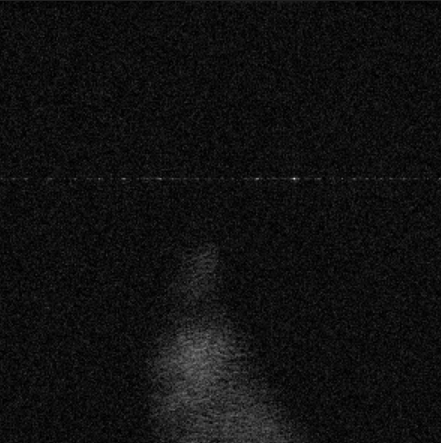
\includegraphics[width=\linewidth]{bad_slice.png}
        \caption{Example of a bad slice.}
        \label{fig:bad_slice}
    \end{minipage}%
    \hfill
    \begin{minipage}{0.45\textwidth}
        \centering
        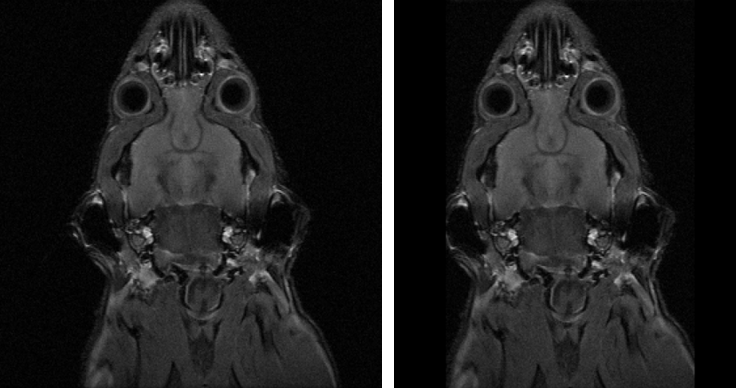
\includegraphics[width=\linewidth]{comparision cropped vs non cropped.png}
        \caption{The left figure shows the original slice, while the right figure is the cropped slice.}
        \label{fig:comparision-cropped}
    \end{minipage}
\end{figure}



\newpage

\section{Appendix: Mathematics APDDM}
\label{appendix:Mathematics APDDM}
\subsection{Ansatz: linear interpolation between image pair}
Some definitions:
\\
$\bold{x}_0$ = high-SNR image\\
$\bold{x}_T^*$ = low-SNR image (* denotes that this is the ground truth endpoint, the reason for this differentiation will be clear later)\\
$T$ = total amount of steps that will be taken\\
t = current timestep in the diffusion path \\
$\alpha_t = \frac{t}{T}$, notation for the fraction of the diffusion path at the current timestep\\
$\bold{R} = \bold{x}_T^* - \bold{x}_0$, the residual\\
\\
Note: $\bold{x}_0$ and $\bold{x}_T^*$ should be normalized images (according to z-score normalization: 
$\frac{x - \overline{x}}{s_n}$), and $\bold{x}_T^*$ should be interpolated to match the size of $\bold{x}_0$.\\
\\
We will start by first defining a procedure, where we linearly interpolate between $\bold{x}_0$ and $\bold{x}_T^*$, and add a not yet specified noise term:
\begin{equation}
    x_t = (1-\alpha_t)\cdot\bold{x}_0 + \alpha_t\cdot\bold{x}_T^* + noise(t)
\end{equation}

\subsection{Proposition of the Markovian process}
We will now transform this into a Markovian process, by allowing the endpoint to not be exactly $\bold{x}_T$, but rather let the endpoint $\bold{x}_T$ be $\bold{x}_T^*$ in expected value.\\
\\
If we subtract $\bold{x}_t$ by $\bold{x}_{t-1}$, we get:
\begin{equation}
    \bold{x}_t - \bold{x}_{t-1} = \alpha_t (\bold{x}_T^* - \bold{x}_0) - \alpha_{t-1} (\bold{x}_T^* - \bold{x}_0) + noise
\end{equation}
$\Leftrightarrow$
\begin{equation}
    \bold{x}_t - \bold{x}_{t-1} = (\alpha_t - \alpha_{t-1}) \bold{R} + noise
\end{equation}
$\Leftrightarrow$
\begin{equation}
    \bold{x}_t = \bold{x}_{t-1} + \frac{1}{T} \bold{R} + noise
\end{equation}
By using a Markov process, we create a natural diffusion path from $\bold{x}_0$ to $\bold{x}_t$, where each step builds up on the previous one. 
We now define our final Markov process as: 
\begin{equation}\label{eq:12}
    \boxed{\bold{x}_t = q(\bold{x}_{t-1}) = \bold{x}_{t-1} + \frac{1}{T} \bold{R} + f(t) \hat{\epsilon} \hspace{.1cm};\hspace{.5cm} t=1,2,...,T}
\end{equation}

Where we define $f(\alpha_t)$ to be a function that is zero for arguments $0$ and $1$, and reaches a maximum of 1 somewhere in the range $[0,1]$. 
This is the noise envelope function. Let:
\begin{equation}\label{eq:13}
    f(t) = 4\alpha_t(1-\alpha_t) = 4 \frac{t}{T} (1-\frac{t}{T})
\end{equation}
This choice of function is arbitrary, but in this way, the noise term is gradually introduced and attenuated again so the course of the diffusion path has a natural way of going from starting point to endpoint. 
Below, the course of the variance throughout the path will be shown, where it will be clear why such a choice of attenuating envelope function is favorable. \\
\\
The noise term $\epsilon$ should be distributed according to the real noise in our data:
\begin{equation}
    \epsilon \sim P[noise]
\end{equation}
We will approximate this empirically by sampling from all the observed residuals in our dataset:
\begin{equation}
    \epsilon \approx \hat{\epsilon} \stackrel{i.i.d.}{\sim} \mathcal{E}_{dataset}
\end{equation}

This sampling of the noise residual can be done by i.i.d sampling residual bank $\mathcal{E}_{dataset}$. These are than rotated at random over 0°, 90°, 180° and 270°. 

\subsection{Expected value of the endpoint}
Note that generally: $\bold{x}_T \neq \bold{x}_T^*$. It will now be shown that the expected value $\mathbb{E}[\bold{x}_T]$ still is $\bold{x}_T^*$:\\
\\
We apply a Markov chain T times to the input $\bold{x}_0$ using \ref{eq:12}:\\
\begin{equation}
    \mathbb{E}[\bold{x}_T] = \mathbb{E}[q(q(...q(\bold{x}_0)..))] = \mathbb{E}[\bold{x}_0 + \frac{T}{T} \bold{R} + \sum_{t=1}^{T} f(t) \cdot \hat{\epsilon}_t] 
\end{equation}
Because $\bold{R}= \bold{x}_T^* - \bold{x}_0$:
\begin{equation}
    \mathbb{E}[\bold{x}_T] = \mathbb{E}[\bold{x}_T^* + \sum_{t=1}^{T} f(t) \cdot \hat{\epsilon}_t] = \bold{x}_T^* + \sum_{t=1}^{T} f(t) \cdot \mathbb{E}[\hat{\epsilon}_t]
\end{equation}
If we assume $\mathbb{E}[\hat{\epsilon}] = 0$:
\begin{equation}
    \boxed{\mathbb{E}[\bold{x}_T] = \bold{x}_T^*}
\end{equation}

\subsection{Variance of the endpoint}
We will now derive the expression for the variance on our endpoint $\bold{x}_T$, again by using \ref{eq:12}:
\begin{multline}
    Var[\bold{x}_T] = Var[q(q(...q(\bold{x}_0)..))] = Var[\bold{x}_0 + \bold{R} + \sum_{t=1}^{T} f(t) \cdot \hat{\epsilon}_t] = \\ \sum_{t=1}^{T} f(t)^2 Var[\hat{\epsilon}_t] + \sum_{i \neq j}^{T} f(i) f(j) Cov[\hat{\epsilon}_i, \hat{\epsilon}_j] = \sum_{t=1}^{T} f(t)^2 Var[\hat{\epsilon}_t]
\end{multline}
Now using the notation: $Var[\hat{\epsilon}_t] = \sigma_{\epsilon}^2$ and \ref{eq:13}, we get:
\begin{equation}
    \boxed{Var[\bold{x}_T] = \sigma_{\epsilon}^2 \cdot \sum_{t=1}^{T} f(t)^2 = \frac{8}{15} \frac{T^4 - 1}{T^3} \cdot \sigma_{\epsilon}^2}
\end{equation}
Note that for $lim_{T->+\infty} Var[\bold{x}_T] \sim \frac{8}{15} T$.\\
\\
We can also derive the general variance throughout the path:
\begin{multline}
    Var[\bold{x}_T] = \sigma_{\epsilon}^2 \cdot \sum_{\tau=1}^{T} f(\tau)^2 = \sigma_{\epsilon}^2 \cdot \frac{8}{15} \frac{1}{T^4} t(t+1)[6t^3 - 15t^2T + 9t^2 + 10tT^2 - 15tT + t + 5T^2 - 1]
\end{multline}
    

% plot -----------------------
\begin{center}
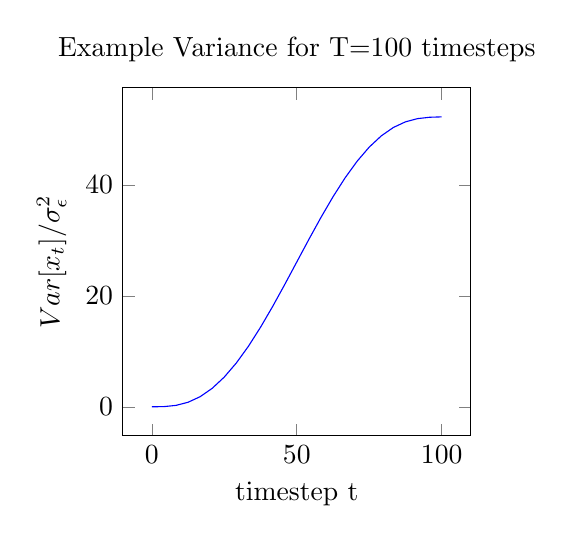
\begin{tikzpicture}
\begin{axis}[ylabel = {$Var[x_t] / \sigma_{\epsilon}^2$}, xlabel={timestep t}, title={Example Variance for T=100 timesteps}, width=6cm, height=6cm]
\addplot[color=blue, domain=0:100]{8/15 * x * (x-1) * 1/(100^4) * (6*x^3 - 15*x^2 * 100 + 9*x^2 + 10*x*100^2 - 15*x*100 + x + 5*100^2 - 1)};
\end{axis}
\end{tikzpicture}
\end{center}

This exact course of the variance has also been confirmed by numerical simulation.\\
\\
We can observe that the variance increases slowly in the beginning, and before the endpoint, it slows down and stabilizes again. 
This is the reason for the particular choice of the envelope function $f(t)$ discussed previously.

\subsection{Controlling the variance}
I will now propose a method of controlling the variance of this path. 
First, we will normalize the sampled residual $\hat{\epsilon}$, so we know the variance of the noise is 1:
\begin{equation}
    \hat{\epsilon'} = \hat{\epsilon} / s_{n,\epsilon}
\end{equation}
($s_{n,\epsilon}$ = population variance of $\mathcal{E}_{dataset}$)\\
Additional note: we assume that an empirical noise distribution has an expected value of 0.\\
We will then control the variance by adding a parameter $\sigma$:
\begin{equation}
    \boxed{\bold{x}_t = q(\bold{x}_{t-1}) = \bold{x}_{t-1} + \frac{1}{T} \bold{R} + \sigma f(t) \hat{\epsilon'} \hspace{.1cm};\hspace{.5cm} t=1,2,...,T}
\end{equation}
Where: 
\begin{equation}
    \sigma = \sqrt{\frac{15}{8} * \frac{T^3}{T^4 - 1}} * \beta
\end{equation}
Now, the variance of our endpoint is: 
\begin{equation}
    Var[\bold{x}_T] = \beta^2
\end{equation}
We now have full control over the variance of the diffusion path.

\subsection{MSE stability}
Important to note is that there are some constraints on this parameter beta (and thus the variance of the noise term), if we want the MSE between $\bold{x}_T$ and $\bold{x}_T^*$ to converge to zero.\\
An important condition that must be met, is that $\bold{x}_t$ becomes more similar to $\bold{x}_T^*$ each step.\\
\\
 This condition will not be met if the noise term overpowers the term $\frac{1}{T}  \bold{R}$. 
 In other words, the residual term magnitude should be larger than the noise term magnitude in each step, so that the diffusion path still mostly converges towards $x_T^*$. 
 We will make an estimation of the size of the subsequent terms based on their Mean Square value $\frac{1}{i,j}\sum_{i,j} X_{i,j}^2$ (MS value). 
 We will also let $f(t) = 1$, to have a conservative estimation.
 The diffusion path will converge if:
\begin{equation}
    \mathbb{E}[MS(\hat{\epsilon})] \lesssim MS(\frac{1}{T} \bold{R})
\end{equation}
$\Leftrightarrow$
 \begin{equation}
    \sigma^2 \cdot MS(\mathbb{E}[\hat{\epsilon}']) \lesssim \frac{1}{T^2} MS(\bold{R})
\end{equation}
$\Leftrightarrow$
 \begin{equation}
    \boxed{\sigma \lesssim \frac{1}{T} RMS(\bold{R}) = \sigma_{crit}}
\end{equation}
This last expression is a conservative MSE convergence condition. \\
In terms of $\beta$:
\begin{equation}
    \beta \lesssim \sqrt{\frac{8}{15} \frac{T^4-1}{T^5}} RMS(\bold{R}) = \beta_{crit}
\end{equation}
\\
This result can be demonstrated by a simulation where beta is varied and the mean square error between $x_T$ and $x_T^*$ is computed over N diffusion path samples (Fig. \ref{fig:beta sweep}). We indeed observe that if $\beta$ is within the order of magnitude of $\beta_{crit}$, the diffusion process won't converge towards $x_T^*$ anymore, which manifests itself in an increase in the MSE. 

\begin{figure}[h]
    \centering
    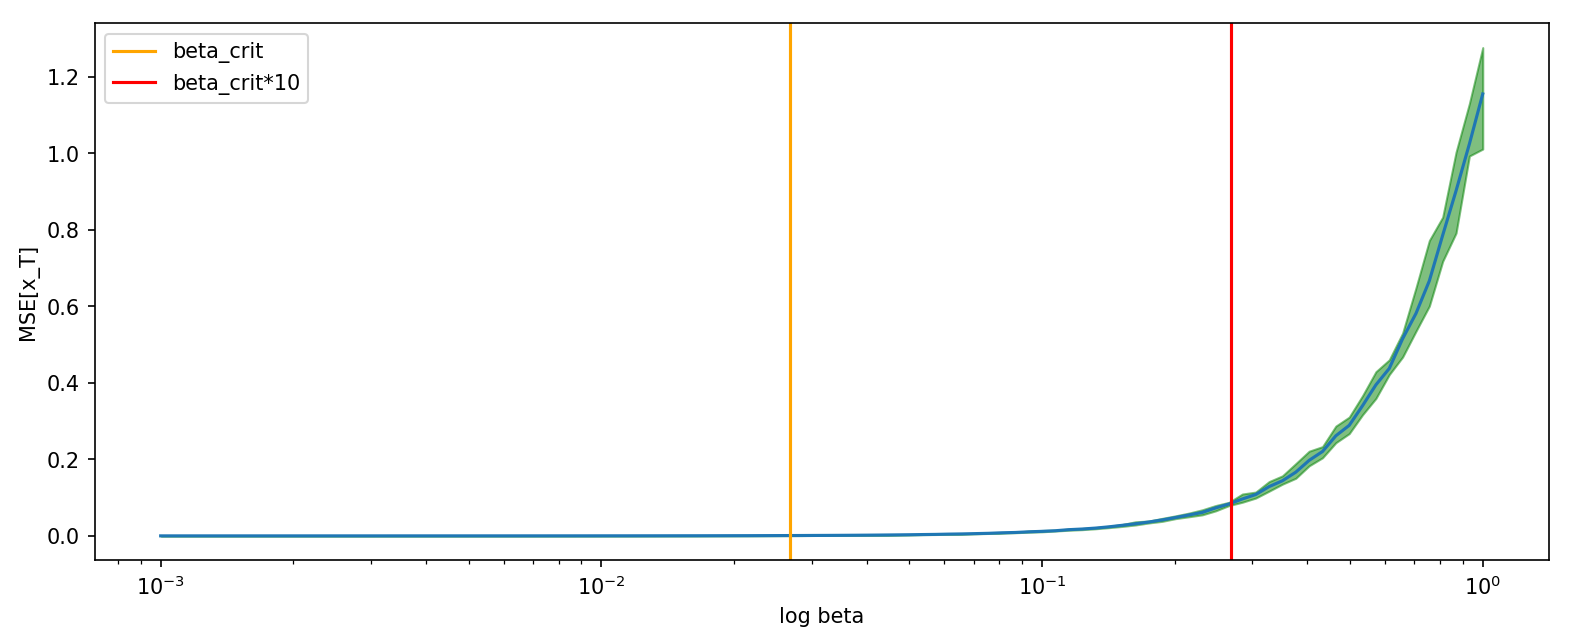
\includegraphics[width=0.8\linewidth]{beta_sweep.png}
    \caption{Plot of $MSE(x_T, x_T^*)$ against beta. }
    \label{fig:beta sweep}
\end{figure}

\FloatBarrier

\newpage
\section{Appendix: Figures Results}
\label{Appendix: Figures Results}
\begin{figure*}[h]
    \centering
    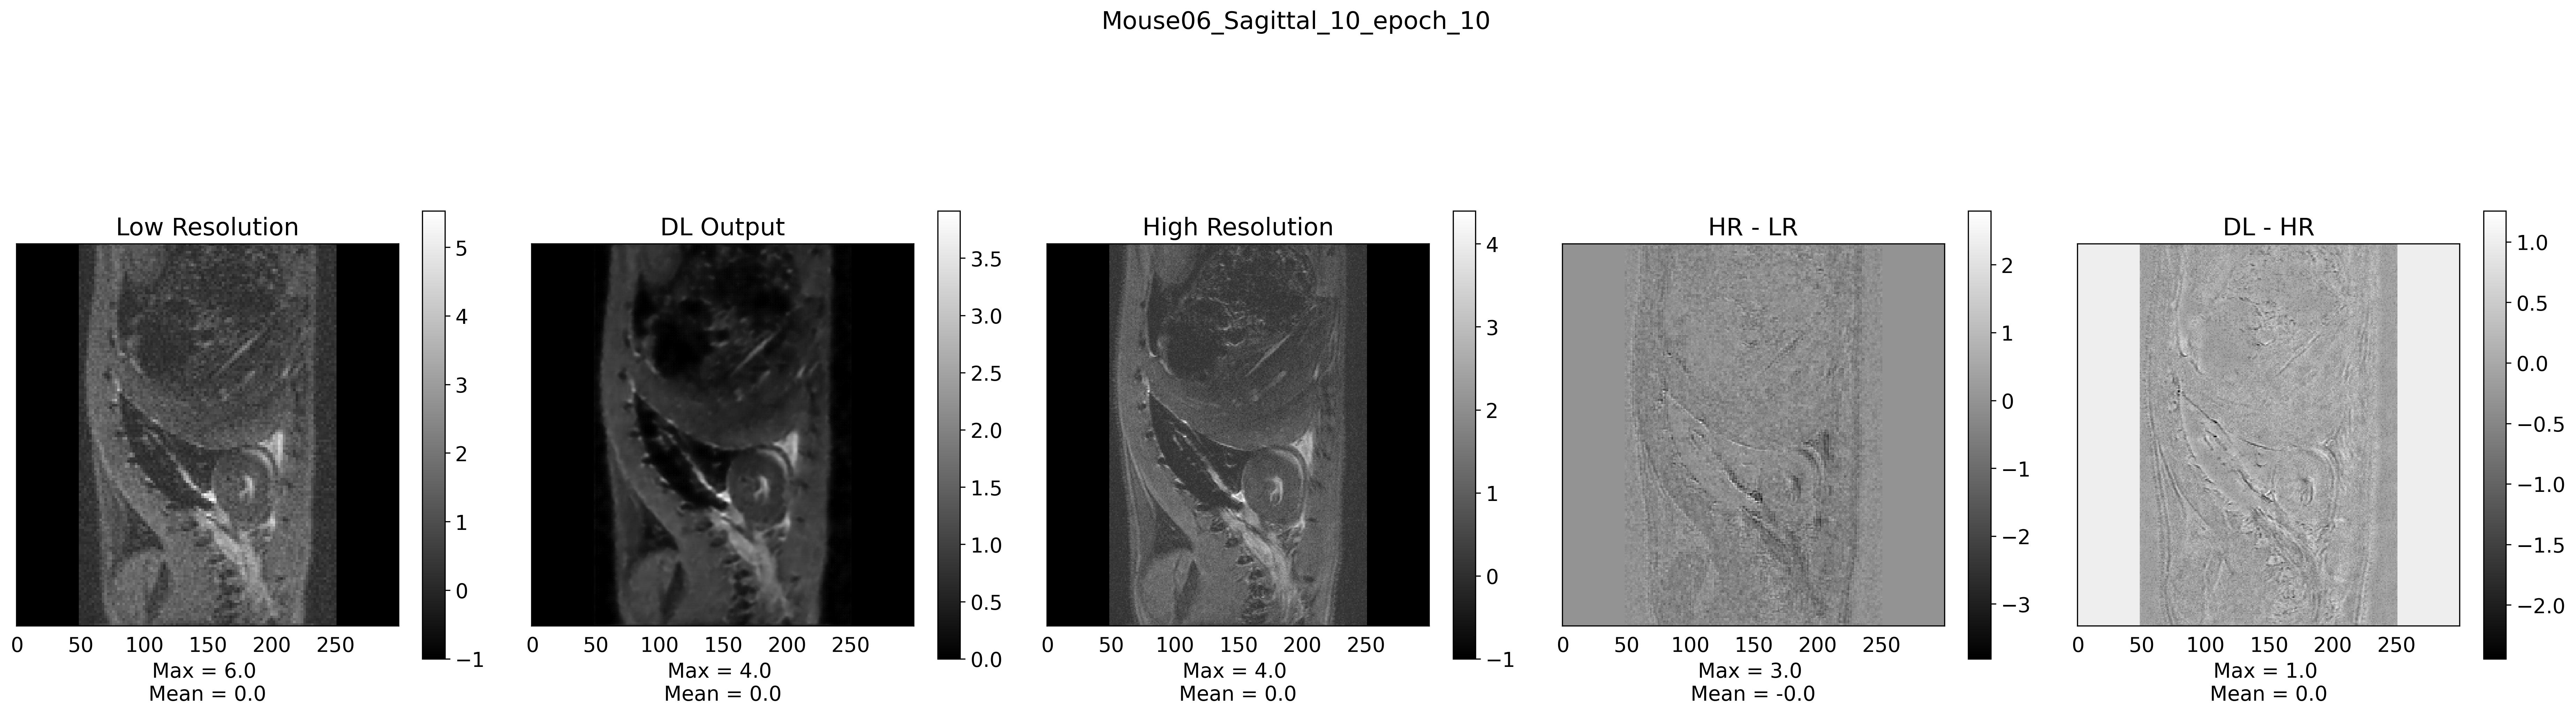
\includegraphics[width=1\linewidth]{Mouse06_Sagittal_10_epoch_10.png}
    \caption{First results of mouse 6 (test) sagittal plane slice 10 after 11th epoch.}
\end{figure*}

\begin{figure*}[h]
    \centering
    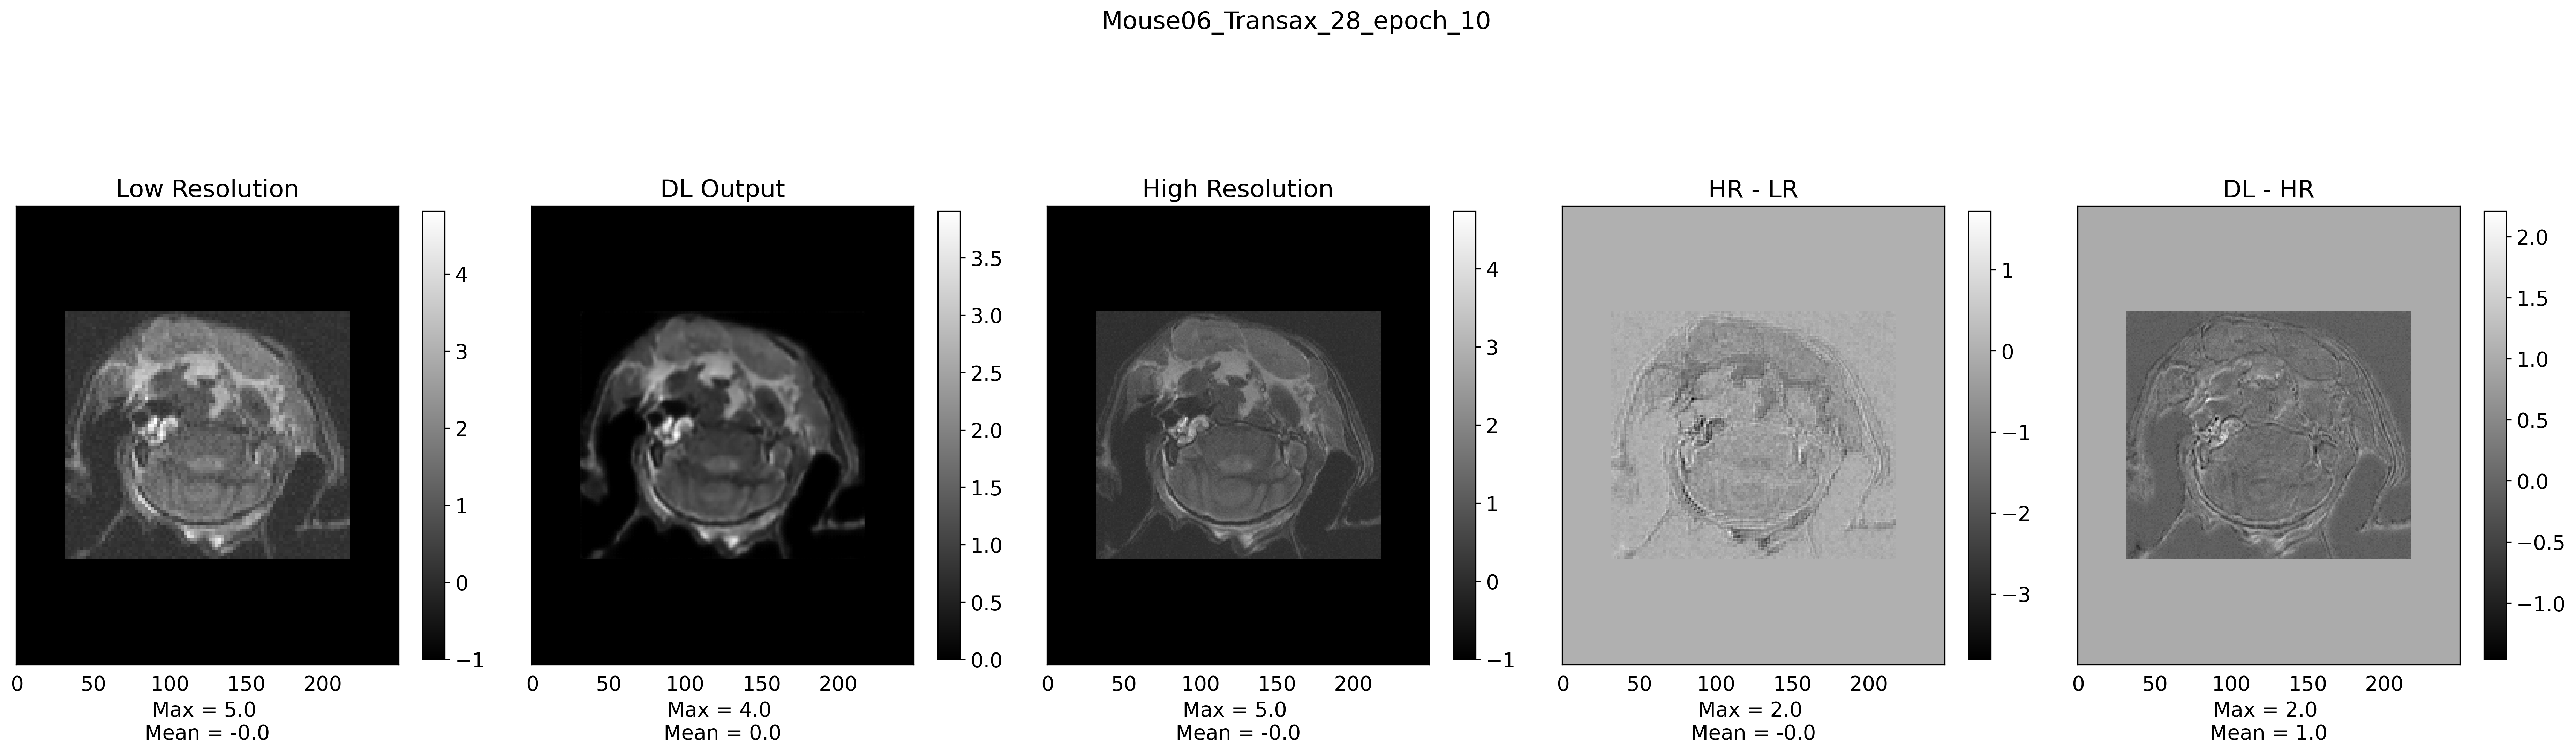
\includegraphics[width=1\linewidth]{Mouse06_Transax_28_epoch_10.png}
    \caption{First results of mouse 6 (test) transaxial plane slice 28 after 11th epoch.}
\end{figure*}

\begin{figure*}[h]
    \centering
    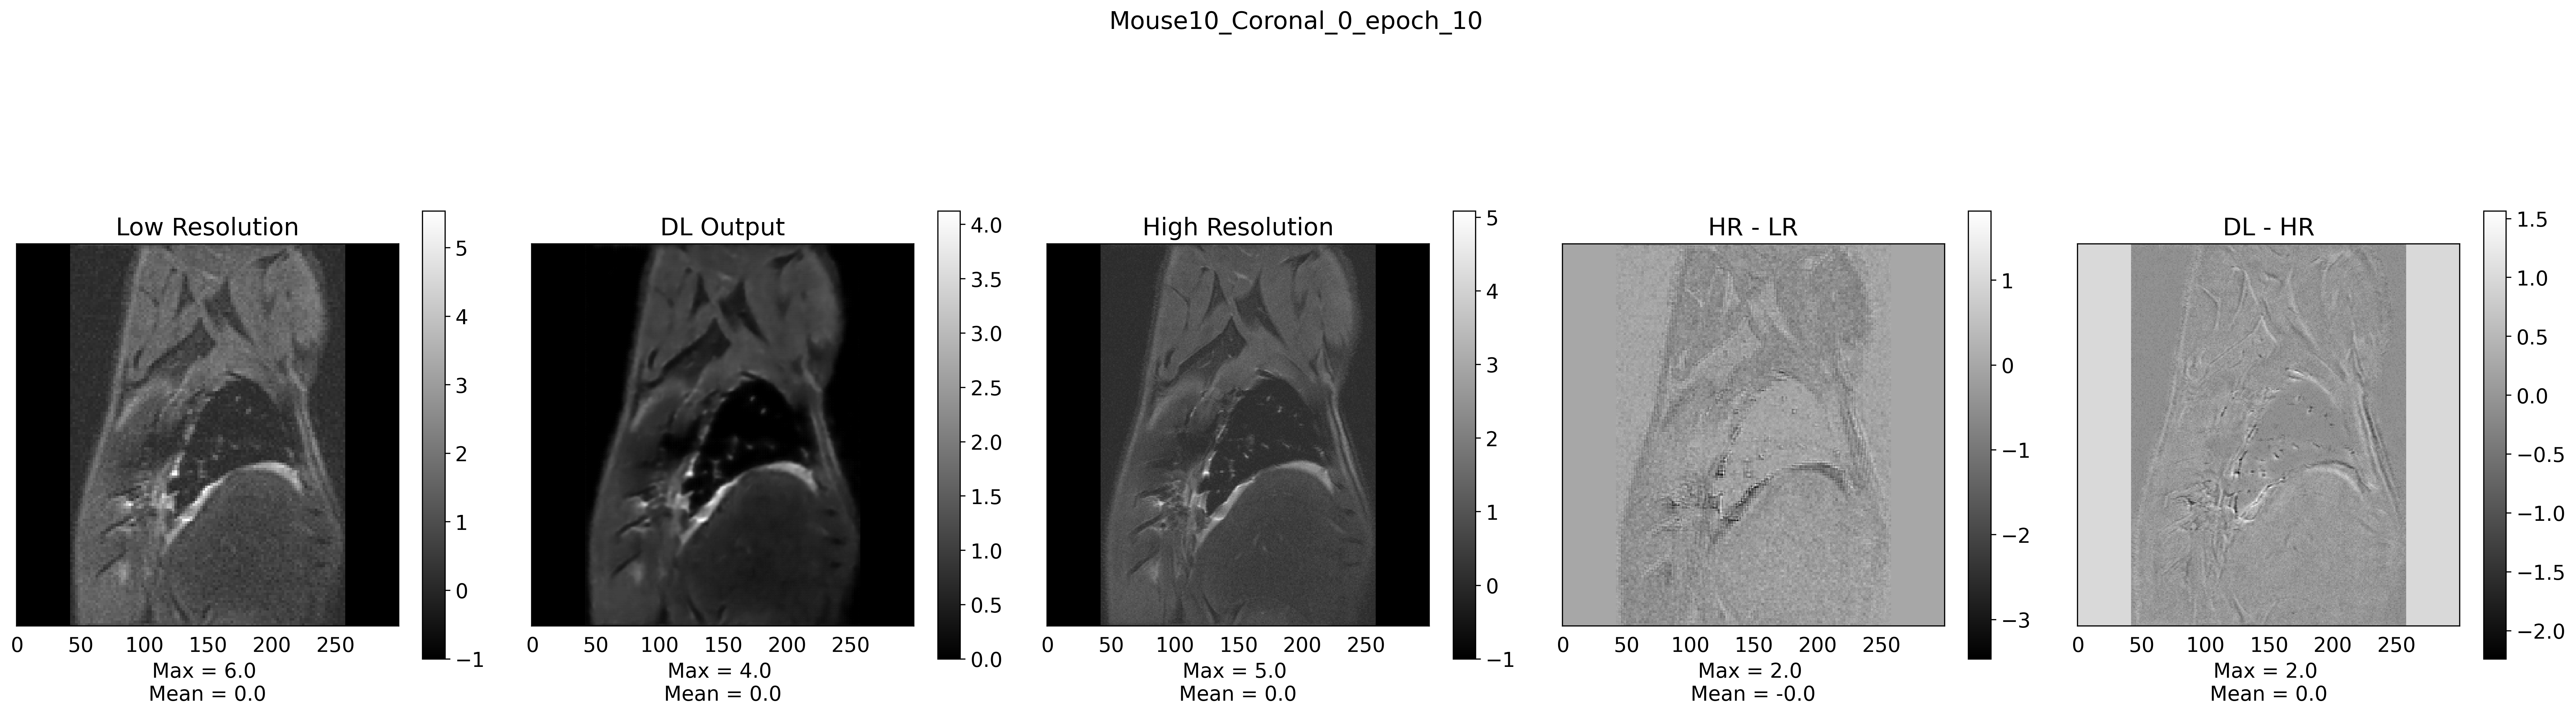
\includegraphics[width=1\linewidth]{Mouse10_Coronal_0_epoch_10.png}
    \caption{First results of mouse 10 (test) coronal plane slice 0 after 11th epoch.}
\end{figure*}


\end{appendices}

\end{document}
